 % \documentclass[acmsmall,screen,review]{acmart}
% \documentclass[10pt,conference]{IEEEtran}

% LLNCS macro package for Springer Computer Science proceedings;
% Version 2.20 of 2017/10/04
%
\documentclass{fmcad}

% \AtBeginDocument{%
%   \providecommand\BibTeX{{%
%     \normalfont B\kern-0.5em{\scshape i\kern-0.25em b}\kern-0.8em\TeX}}}

% \usepackage{natbib}
\usepackage{amsmath}
\interdisplaylinepenalty=2500
\usepackage{amssymb}
\usepackage{algorithm}
\usepackage{algorithmicx}
\usepackage{algpseudocode}
\usepackage{paralist}
\usepackage[shortlabels]{enumitem}
\usepackage{xcolor}
\usepackage{xspace}
\usepackage{listings}
\usepackage{hyperref}
\usepackage{cleveref}
\usepackage{latexsym}
\usepackage{colortbl}
\usepackage{graphicx}
\usepackage{comment}
\usepackage{booktabs}
\usepackage{multirow}
\usepackage[export]{adjustbox}
\usepackage{tikz}
\usepackage{dcolumn}
\usepackage{mathspeak}


%% Rights management information.  This information is sent to you
%% when you complete the rights form.  These commands have SAMPLE
%% values in them; it is your responsibility as an author to replace
%% the commands and values with those provided to you when you
%% complete the rights form.
% \setcopyright{acmcopyright}
% \copyrightyear{2024}
% \acmYear{2024}
% \acmDOI{XXXXXXX.XXXXXXX}

%%
%% These commands are for a JOURNAL article.
% \acmJournal{JACM}
% \acmVolume{37}
% \acmNumber{4}
% \acmArticle{111}
% \acmMonth{8}

\usetikzlibrary{positioning}
% \citestyle{acmauthoryear}


\newcommand\SI[1]{{\color{purple}{SI: #1}}}
\newcommand\ES[1]{{\color{blue}{ES: #1}}}


\newcommand\eg{\textit{e.g.}\@\xspace}
\newcommand\ie{\textit{i.e.}\@\xspace}
\newcommand\vs{\textit{vs.}\@\xspace}

\newcommand\funcname[1]{\textsf{\fontsize{8.5pt}{8pt}\selectfont#1}}
\newcommand\smallfuncname[1]{\textsf{\fontsize{7.5pt}{7pt}\selectfont#1}}

\newcommand\ecid[1]{\langle #1\rangle}

\newcommand\tfilter{\funcname{filter}}
\newcommand\tmax{\funcname{max}}
\newcommand\tmin{\funcname{min}}
\newcommand\ttrue{\funcname{true}}
\newcommand\tfalse{\funcname{false}}
\newcommand\tissorted{\funcname{is\_sorted}}
\newcommand\tbinsearch{\funcname{bin\_search}}
\newcommand\tlfind{\funcname{find}}

\newcommand\tsmallmax{\smallfuncname{max}}
\newcommand\tsmallmin{\smallfuncname{min}}

\newcommand\tif{\mathrm{if}}
\newcommand\tthen{\mathrm{then}}
\newcommand\telse{\mathrm{else}}

\newcommand\apifun[1]{\mathit{#1}}
\newcommand\tunion{\apifun{union}}
\newcommand\tfind{\apifun{find}}
\newcommand\tinsert{\apifun{insert}}
\newcommand\tmerge{\apifun{merge}}

\definecolor{olivegreen}{HTML}{3C8031}

\newcommand\croot{\ensuremath{\varnothing}\xspace}
\newcommand\cblue{{\color{blue}blue}\xspace}
\newcommand\cred{{\color{red}red}\xspace}
\newcommand\cgreen{{\color{olivegreen}green}\xspace}

\newcommand\tterm{\mathit{term}}
\newcommand\treg{\mathit{reg}}
\newcommand\tin{\mathit{in}}
\newcommand\tout{\mathit{out}}
\newcommand\trevpath{\mathit{reverse\_path}}
\newcommand\tcolor{\mathit{color}}
\newcommand\teclass{\mathit{eclass}}
\newcommand\tdescendants{\mathit{descendants}}
\newcommand\tminimal{\mathit{minimal}}

\newcommand\instr[1]{{\fontsize{9.5pt}{8pt}\selectfont\textsf{#1}}}
\newcommand\iinit{\instr{init}}
\newcommand\ibind{\instr{bind}}
\newcommand\icompare{\instr{compare}}
\newcommand\icheck{\instr{check}}
\newcommand\icontinue{\instr{continue}}
\newcommand\ijoin{\instr{join}}
\newcommand\iclrjmp{\instr{colored\_jump}}

\newcommand\rwto{\overset{.\,}{\rightarrow}}

\newcommand\congblue{{~\color{blue}\cong_{\mathrm{b}}\,\,}}
\newcommand\congred{{~\color{red}\cong_{\mathrm{r}}\,\,}}
\newcommand\conggreen{{~\color{olivegreen}\cong_{\mathrm{g}}\,\,}}

\newcommand\congbluesym{{\color{blue}\cong_{\mathrm{b}}}}


\newcommand\lowerred{{\color{red}_{\hspace{1pt}\mathrm{r}\hspace{0.5pt}}}}

\newcommand\eqid{\equiv_{\mathrm{id}}}
%
\newcommand\myparagraph[1]{
  \smallskip\noindent\textbf{#1}~}

\newcommand*{\algorithmautorefname}{Algorithm}

% because autoref does not work with the fmcad/IEEE class
\newcommand{\annexref}[1]{\hyperref[#1]{Appendix~\ref*{#1}}}

% Define a boolean flag for anonymization
\newif\ifanon
\anontrue  % Uncomment this line to enable anonymization
%\anonfalse % Uncomment this line to disable anonymization

% Define the anonymization macro
\newcommand{\annon}[1]{%
    \ifanon
        [Anonymized]%
    \else
        #1%
    \fi
}

\makeatletter
\NewDocumentCommand{\LeftComment}{O{0em} m}{%
  \Statex \hspace*{\ALG@thistlm}\hspace{#1}\(\triangleright\) #2}
\makeatother

% \bibliography{refs}

\lstdefinestyle{codestyle}{
    keywordstyle={\bfseries}, 
    commentstyle={\color{codegreen}},
    stringstyle=\color{codepurple},
    basicstyle=\ttfamily\footnotesize,
    numbers=left, 
    language=Python 
} 
\lstset{style=codestyle}


\begin{document}

%\titlerunning{Easter Egg: Equality Reasoning with Multiple Assumptions}
\title{Easter Egg: Equality Reasoning Based on E-Graphs with Multiple Assumptions}

% \author{Eytan Singher}
% \email{eytan.s@cs.technion.ac.il}
% \affiliation{%
%   \institution{Technion}
%   \city{Haifa}
%   \country{Israel}
% }
% \author{Shachar Itzhaky}
% \email{shachari@cs.technion.ac.il}
% \affiliation{%
%   \institution{Technion}
%   \city{Haifa}
%   \country{Israel}
% }
% \author{Eytan Singher and Shachar Itzhaky}

\author{\IEEEauthorblockN{Eytan Singher and Shachar Itzhaky}
\IEEEauthorblockA{
  Technion - Israel Institute of Technology, Haifa, Israel
}
}
% \author{Eytan Singher\inst{1}\orcidID{0009-0008-4020-9040} \and
% Shachar Itzhaky\inst{1}\orcidID{0000-0002-7276-7644}}

% \institute{Technion Israel Institute of Technology, Haifa 3200, Israel
% \email{eytan.s,shachari@technion.ac.il}\\
% \url{https://cs.technion.ac.il/}}

%\email{Anonymous}\\
%\url{Anonymous}}

\maketitle

\begin{abstract}
% Intro: E-graphs are awsome and especially when used for equality saturation
% Motivation: Exploratory reasoning tasks + equality saturation will be stuck on case splits 
% Solution: Multiple congruence relations in a singhle e-graph
% Contributions: colored e-graph approach + implementation. Experiments
% Results are good

E-graphs are a prominent data structure that has been increasing in popularity in recent years due to their expanding range of applications in various formal reasoning tasks.
E-graphs allow systematic and efficient treatment of equality, which is pervasive in automated
reasoning based on proofs.

E-graphs handle equality well, but are severely limited in their handling of case splitting and other aspects of propositional reasoning, such as resolution, which introduce branching in provers and solvers.
As a consequence, most tools resort to using e-graphs locally, recreating them ad-hoc when they are needed, and then discarding them.
In exploratory scenarios, where it is necessary to retain multiple branches simultaneously, this limitation proves to be prohibitive.
In particular, in theory exploration---%
a process where lemmas are discovered and then proven---this poses a significant challenge.
Theory exploration must enumerate a space of possible assumptions, and must retain all of them
to make progress.
This poses a severe limitation on the ability to harness e-graphs for the task.

Our key observation is that in exploratory reasoning tasks, branching represents versions of the same e-graph each with an added assumption, such as ``$x > y$'' or ``$\tissorted\,l$''.
Essentially, each e-graph represents an equality relation, and each branch corresponds to a matching coarsened equality relation.
Based on this observation, we present an extension to e-graphs, called \emph{Colored E-Graphs}, as a way to efficiently represent all of the coarsened equality relations in a single structure.
A colored e-graph is a memory-efficient equivalent of multiple copies of an e-graph, with a much lower overhead.
This is attained by sharing as much as possible between different cases, while carefully tracking which conclusion is true under which assumption.
It can be viewed as adding multiple ``color-coded'' layers on top of the original e-graph structure, representing different assumptions.

We run experiments and demonstrate that our colored e-graphs can support large numbers of assumptions and terms with space requirements that are about $10\times$ lower, and with slightly improved performance.

%\keywords{Automatic reasoning \and Theory exploration \and E-graph.}

\end{abstract}


% Old version
\begin{comment}
% E-graphs are cool and getting prominent                 }
% E-graphs do equality saturation in other words          } E-graphs are interesting
% They are useful for formal methods                      }
% Problem - Boolean structures
% 

E-graphs are a prominent data structure that has been increasing in popularity in recent years, with a growing number of uses in formal methods and programming languages.
% Used in programming languages: different papers for optimizing code, and for algebric computation in julia
E-graphs excel at drawing consequences from a set of universally quantified equality formulas via repetitive application of first-order equality axioms.
They offer powerful automated reasoning tools such as e-matching and e-unification, that can be used for automated theorem proving and verification.
An aspect in which they lack relative to other proving techniques, such as resolution and sequent calculi, is handling arbitrary Boolean structure in first-order formulas.

In this work, we develop an extension to e-graphs to allow them to be able to support formulas in the form of logical implications. This is done by introducing conditional conclusions that are distinguished according to the implicant; different assumptions may give rise to different conclusions, and in the context of exploratory reasoning (such as proof search and lemma synthesis), it is desired to have an efficient way to store them all simultaneously.

In this context, we have identified that memory becomes a major bottleneck, and may quickly cause a reasoning to run out of memory and be unable to complete the task as hand. \SI{todo}  
We demonstrate that our Colored E-graphs can support a multitude of assumptions with an order of magnitude lower space requirements, and with similar time requirements.

\end{comment}

% \begin{CCSXML}
<ccs2012>
   <concept>
       <concept_id>10011007.10011074.10011099.10011692</concept_id>
       <concept_desc>Software and its engineering~Formal software verification</concept_desc>
       <concept_significance>300</concept_significance>
       </concept>
 </ccs2012>
\end{CCSXML}

\ccsdesc[300]{Software and its engineering~Formal software verification}

% \keywords{Do, Not, Us, This, Code, Put, the, Correct, Terms, for,
%   Your, Paper}

% \thispagestyle{plain}
\pagestyle{plain}
\section{Introduction}
\label{colors:intro}

% Context
E-graphs are a versatile data structure that is used for various tasks of automated reasoning, including theorem proving and synthesis.
E-graphs have been popularized in compiler optimizations thanks to their ability to support efficient \emph{rewrites} over a large set of terms, while keeping a compact representation of all possible rewrite outcomes.
This mechanism is known as \emph{equality saturation}.
It provides a powerful engine that allows a reasoner to generate all equality consequences of a set of known, universally quantified, equalities.
Possible uses include selecting the best equivalent of an expression according to some desired metric, such as run-time efficiency~\cite{eqsat}, size~\cite{flatt2022small,DBLP:conf/fmcad/NotzliBNPRBT22}, or precision~\cite{herbie}
(when used as a compilation phase)
and a generalized form of unification, called e-unification, for application of inference steps (when used for proof search).

In this work we focus on a stepping stone for what we address as \emph{exploratory reasoning}: a range of tasks including all the above optimization procedures, as well as theory exploration \cite{thesy}, rewrite rule inference \cite{ruler}, and proof search \cite{vampire,DBLP:conf/aplas/BrotherstonGP12,cycleq}.
Exploratory reasoning, in general, can be thought of as any reasoning task navigating a large space of potential goals or sub-goals that need to be selected based on some criteria.
Our motivating example comes from TheSy and Ruler, both of which are theory exploration systems based on e-graphs. 
A theory exploration system attempts to both discover and prove mathematical properties from a set of definitions and known lemmas.
Most of the difficulty in theory exploration comes from the generation and filtering of candidates, rather then from the proof procedure itself.
TheSy does so by efficiently filtering a large set of potential conjectures using e-graphs for equality reasoning, and evaluating which should be potentially proved.
While e-graphs are effective for equality reasoning \cite{egg}, handling branching, such as case splitting during proof search, do not have a common solution, and are treated ad-hoc.
For example, a special type of node is introduced in \cite{eqsat} to deal with loop conditions, while in \cite{coward2023automating} a special operator is introduced to reason on expressions under certain contexts, and \cite{thesy} creates full copies of the e-graph for each branch being explored.

% Gap
To illustrate this difficulty, we zoom in on an example from theory exploration.
As an example scenario, consider trying to discover and prove lemmas on sorted lists:
a library containing functions $\tlfind$, $\tissorted$, and $\tbinsearch$.
We expect to discover lemmas involving these functions; one such lemma might be the property: $\tissorted\,l \rightarrow \tbinsearch\, l\,v = \tlfind\,l\,v$.
State-of-the-art theory exploration systems~\cite{ITP2017:Johansson,ruler,thesy} have some enumeration strategy over expressions in order to discover candidates. 
A challenge presents itself when some lemmas in the space require an assumption, in this case $\tissorted\,l$.
When dealing with e-graphs,
adding an assumption would \emph{globally}
affect all terms involved in the enumeration, making it impossible to separate conclusions stemming from different assumptions.
Because the system cannot know in advance which assumptions will become relevant for discovering equalities, it is required that it also generate and test multiple candidate assumptions.
An immediate solution is to create one copy of the graph per assumption, but doing so can significantly increase the memory usage.
Moreover, lemmas may depend on one another; for example, $\tissorted\,l \rightarrow \tbinsearch\, l\,v = \tlfind\,l\,v$ depends on transitivity of $\leq$ ($x\leq y \land y\leq z \rightarrow x\leq z$).
Therefore, just trying the candidates one at a time would mean that the system would prematurely discard candidates depending on the order in which they are tested; alternatively, for each candidate that is validated and becomes a lemma, it would be forced to re-try all the previously failed attempts, which is highly costly.

% Theory exploration systems based on random testing  (\todo{speculate, hipspec with conditions}) attempt to greedily discover

% Innovation
To overcome this difficulty, we propose an extension of the e-graph data structure.
An e-graph naturally represents a congruence relation $\cong$, which is an equivalence relation over terms (with function applications), which  maintains $x \cong y \vdash f(x) \cong f(y)$ (see \autoref{perlims:congrel}).
The congruence relation is maintained in the e-graph as a set of equivalence classes (e-classes), which can be merged as part of updating the underlying relation. 
We extend the e-graph data structure into a \emph{Colored E-Graph} to maintain multiple congruence relations at once, where each relation is associated with a color.
Our key observation is that each added assumption, can be treated as a new congruence relation, but is only a coarsening of the original relation. 
The coarsening, then, can be represented as a set of additional merges of e-classes on top of the original e-graph.
The main benefit is reducing memory consumption by re-using and sharing most of the e-classes between colors.
Going back to the sorted list example, in the colored e-graph there will be a \cred relation for assuming $x \le y \land y \le z$, and a \cblue relation for assuming $\tissorted\,l$.
Thanks to the size reduction, multiple relations can exist at once, and thus the lemma $\tissorted\,l \rightarrow \tbinsearch\, l\,v = \tlfind\,l\,v$ can be discovered after transitivity of $\leq$ is proven, but without dependency on the order of exploration.
Colored e-graphs also support having a hierarchy between different colors, which can benefit from additional sharing of e-classes.
For example, the \cred color representing $x \le y \land y \le z$ is itself a coarsening of some \cgreen color representing just the assumption $x \le y$.

While the memory footprint for each color is smaller, maintaining the congruence relation and the data structure invariants becomes more challenging.
To address this we present specialized data-structure modifications and evaluate them.
%We also extend the colored e-graph's logic in several key ways, to support e-graph operations for all the colors.
First, we set up a multi-level union-find where the lowest level corresponds to the root congruence.
Second, we change how congruence closure is applied to the individual congruence relations while taking advantage of the sharing between each such relation and the root. 
Lastly, we present a technique for efficient e-matching over all the relations at once.

% Oh we are so good!
\medskip
Our contributions are:
\begin{enumerate}[leftmargin=1.1em]
    \item The observation that assumptions induce coarsened e-graphs that share much of the original structure. 
    \item Algorithms for colored e-graphs operations.
    \item Optimizations on top of the basic algorithms to significantly improve resource usage.
    \item A colored e-graph implementation, \emph{Easter Egg}\footnote{\url{https://github.com/eytans/egg/tree/features/color_splits}} and an evaluation that shows an improvement factor in memory usage over the existing baseline, while maintaining similar run-time performance.
\end{enumerate}
% \section{Background}
\label{lweqsat:background}

Proof assistants usually consist of two basic layers: a \emph{kernel} is responsible for checking proofs, and some user facing scripting language, commonly called a \emph{tactic language} that is used to ease and streamline the construction of proof objects that are passed to the kernel for checking.
This split is conducive to the evolution of proof assistants, because the tactics can be developed more flexibly, without worrying about proof soundness.
The kernel alone forms the TCB (trusted code base) that is assumed correct.

Two of the most commonly used proof assistants today, Coq and Lean \ES{cite}, are based on Type Theory, thus reducing the problem of proof checking to one of \emph{type checking}.
They employ similar flavors of the Calculus of Inductive Constructions (CIC), which is a typed pure lambda calculus with polymorphism and, importantly, dependent types.
In such calculi, types are first-class expressions, and 
type checking relies heavily on syntactic unification of terms.
To offer some automatic assistance, terms are reduced to a \emph{normal form} and then compared.
The normalization relies on the set of reductions that are part of the calculus (the most basic ones being $\beta$-reduction and $\eta$-reduction),
as well as on definitions of basic mathematical concepts that are used (such as arithmetic operators like $+$ and $\cdot\,$).

%(modulo $\beta$-equivalence).
%Terms that are not syntactically identical but are nevertheless semantically equivalent, such as $x\cdot 5$ and $5\cdot x$, require manual application of the tactic language to show equality.

\subsection{Hammer Systems}

Hammer systems have emerged as powerful tools for automating proof discovery in ITPs. These systems typically combine premise selection, translation to first-order logic, and proof reconstruction. Notable examples include Sledgehammer for Isabelle/HOL \cite{sledgehammer}, HOLyHammer for HOL Light \cite{holyhammer}, and CoqHammer for Coq \cite{coqhammer}. These systems have demonstrated significant success in automatically proving a substantial portion of theorems in their respective libraries.

\subsection{Translations to First-Order Logic}

A key component of hammer systems is the translation of higher-order or dependently typed logics to first-order logic. This translation enables the use of highly optimized automated theorem provers (ATPs) that operate on first-order logic. Significant work in this area includes:

\begin{itemize}
    \item Czajka's shallow embedding of pure type systems into first-order logic \cite{czajka2018shallow}, which provides a foundation for translating dependently typed systems.
    \item Meng and Paulson's technique for translating higher-order clauses to first-order clauses \cite{meng2008translating}, which has been influential in the development of hammer systems for higher-order logic.
\end{itemize}

These translations face the challenge of balancing completeness, soundness, and practical efficiency.

\subsection{Automation in Dependently Typed Systems}

Dependently typed proof assistants like Coq and Lean have their own built-in automation tactics. Coq provides tactics such as \texttt{auto}, \texttt{eauto}, and \texttt{firstorder} \cite{Coq:manual}, which perform limited proof search. Lean offers a powerful tactic framework that allows users to write custom automation \cite{lean}.

Integration with SMT solvers has also been explored, as exemplified by Armand et al's work \cite{armand2011modular}, which integrates SMT solvers into Coq's by using proof witnesses, as opposed to hammers which attempt to reconstruct proofs using deductions.

\subsection{Premise Selection}

Efficient premise selection is crucial for the performance of hammer systems, especially when dealing with large formal libraries. Recent advancements in this area include the use of machine learning techniques. For instance, \ES{TODO}.

\subsection{Equality Saturation}

Equality saturation, implemented efficiently using e-graphs, has shown promise in program optimization and equivalence reasoning \cite{egg}. This technique allows for a more flexible exploration of the equality relation, potentially offering advantages in proof search and simplification.

Our work builds upon these foundations, aiming to develop a lightweight equality saturation approach for Coq that balances automation power with logical soundness and efficiency.
\section{Overview}
\label{chap:colored-egraph}
\label{colors:overview}

% <The story goes:>
% 1. Connect motivation (from intro) to egg (as described in background), highlight uses in TheSy (and ruler)
% 2. General concept of colored (layered) e-classes
%    2.a. Explain clone semantics and how colored e-classes are equivalent
% 3. What e-graph operations need to be modified to support colored e-classes
% 4. Challenges and problems (performance bottlenecks caused by the new design)
% 5. Summary of optimization (primer for next section)

\begin{figure}[t]
  \centering
\begin{comment}
  \node(black)[label={above:$\cong$},
               label={[sub]below:{\small (a)}}] {
  %$\cong$ & $\congblue$ & $\congred$ \\
    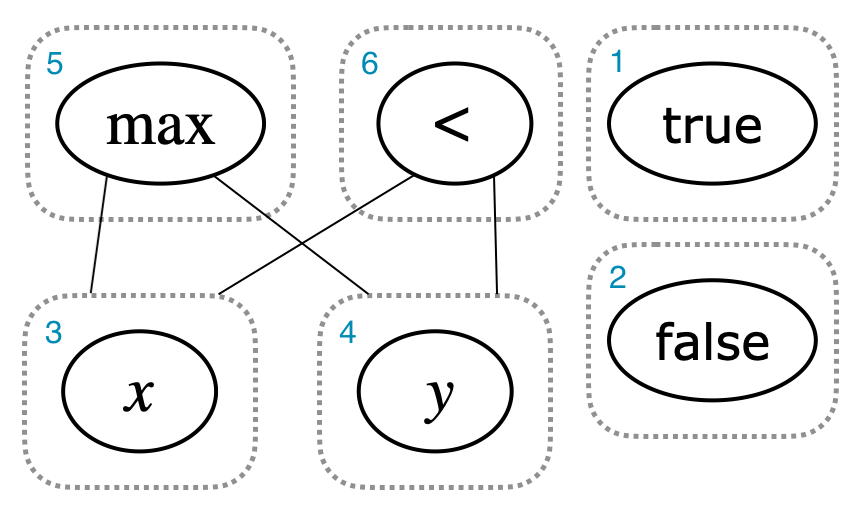
\includegraphics[width=2.7cm,valign=c]{gfx/egraph-max.png}
  };
\end{comment}

  \begin{tikzpicture}[sub/.style={label distance=0,outer sep=0,inner sep=0}]
  \node(blue) [label={[sub]above:$\congblue\!\!$},
               label={[sub]below:{\small (a)}}] {
    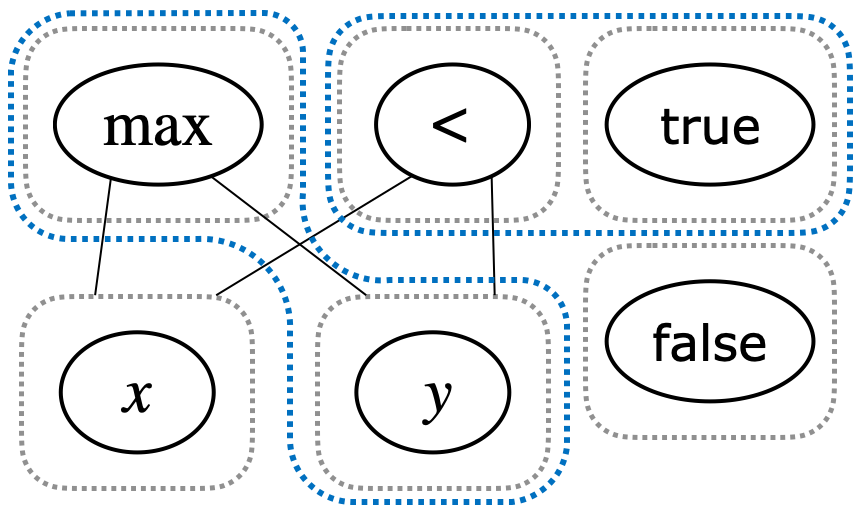
\includegraphics[width=2.7cm,valign=c]{colors/gfx/egraph-max-blue.png}    
  };
  \node(red)[right=0mm of blue,
             label={[sub]above:$\congred$},
             label={[sub]below:{\small (b)}}] {
    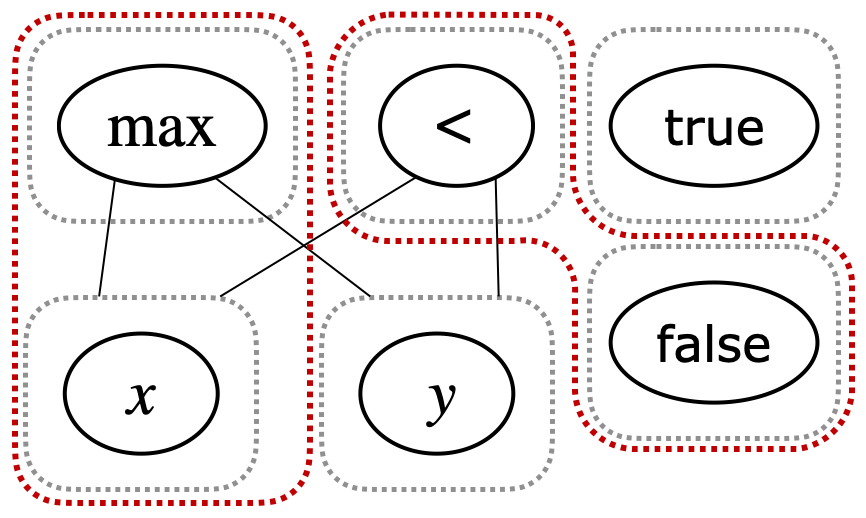
\includegraphics[width=2.7cm,valign=c]{colors/gfx/egraph-max-red.png}
  };
  \node(mixed)[right=0mm of red,
               label={[sub]below:{\small (c)}}] {
    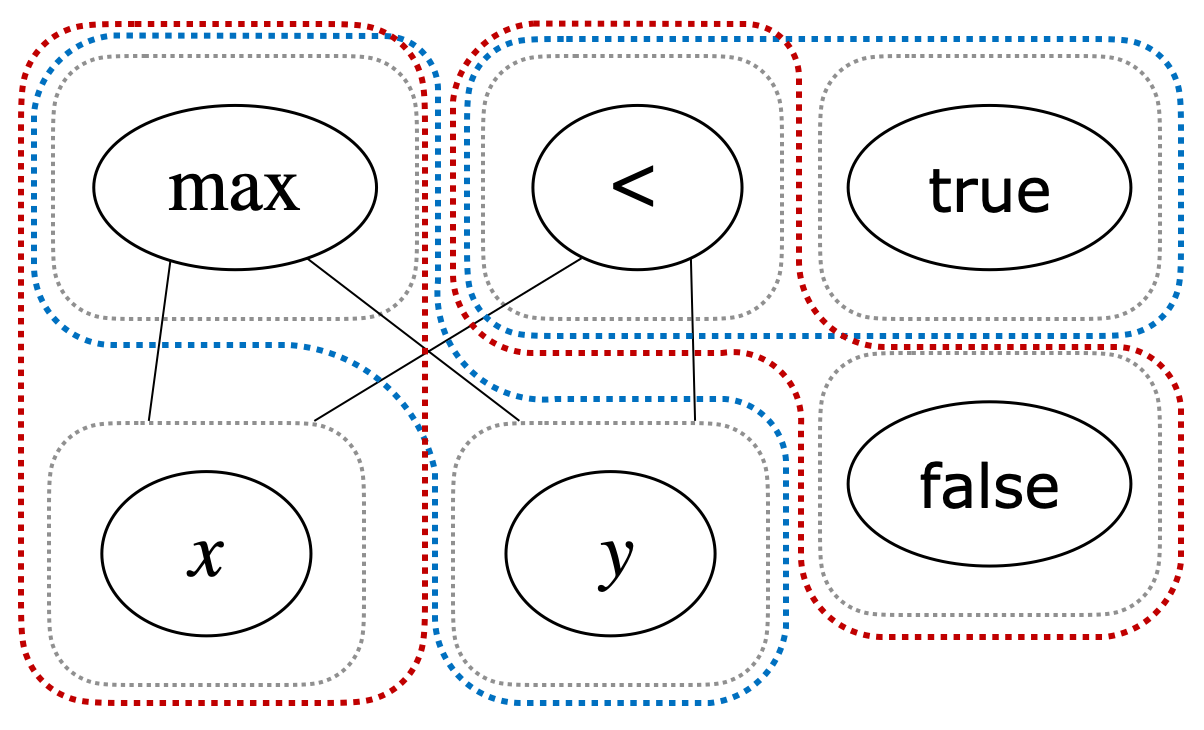
\includegraphics[width=2.9cm]{colors/gfx/egraph-max-red-blue.png}  
  };
  \end{tikzpicture}
  \vspace{-1.5em}
  \caption{Example e-graph with two colored layers; (a) is blue, (b) is red, (c) shows them combined.}
  \label{overview:egraph-max}
\end{figure}

From this point we assume familiarity with the basic e-graph structure which includes a union-find, hashcons, and an e-class map, as well as the basic operations of add, merge, rebuild, and e-matching (and consequently rewriting).
For readers unfamiliar with e-graphs, or with deferred rebuilding, which was introduced in \cite{egg}, additional background is given in  \annexref{background}. \ES{todo put in some real background}

\emph{Colored E-graphs} are an extension of e-graphs devised to add a generic approach for supporting conditional reasoning to e-graphs.
Existing exploratory reasoning systems such as TheSy~\cite{thesy} and Ruler~\cite{ruler} utilize equality saturation with e-graphs for discovering new rewrite rules, but are limited in the presence of conditionals.
For example, let $t := \tmax(x, y)$, then reasoning about the cases $x < y$ and $x \geq y$ separately is desirable: in the first case $t \cong x$, and in the second $t \cong y$.
Without any assumptions, we can say neither and rewriting of $t$ is blocked.
The approach in \cite{thesy} involves a prover that creates an e-graph \emph{clone} for each case in case splitting, such as for $x < y$ and $x \geq y$. 
This process, however, incurs high runtime and memory costs. 
Non-relevant terms in the e-graph are unnecessarily duplicated, and rewrites are redundantly applied to these copies. 
Further case splits compound this issue, leading to an exponential increase in the number of clones with additional nested splits.

%\ES{represent colored e-graphs shortly because it was last seen in the intro}

Colored e-graphs are designed to avoid duplication via sharing of the common terms, thus storing them only once when possible.
The e-graph structure becomes \emph{layered}:
the lowermost layer represents a congruence relation over terms that is true in all cases (represented, normally, as e-classes containing e-nodes).
On top of it are layered additional congruence relations that arise from various assumptions.


Going back to our example, the corresponding e-graph is
shown in \autoref{overview:egraph-max},
containing the terms $\tmax(x, y)$, $x < y$, $\ttrue$ and $\tfalse$.
Layers corresponding to assumptions $x < y$ and $x \geq y$ are shown in \ref{overview:egraph-max}(a) and \ref{overview:egraph-max}(b).
To evoke intuition, we associate with each layer a unique \emph{color}, and paint their e-classes (dotted outlines, in depicted e-graphs) accordingly.
Conventionally, the lowermost layer is associated with the color black.
In the subsequent example we will use \cblue for $x<y$ and \cred for $x\geq y$ when referring to the example.
In the \cblue layer, $(x < y) \congblue \ttrue$ and
$\tmax(x, y) \congblue y$;
in the \cred layer, $(x < y) \congred \tfalse$
and $\tmax(x, y) \congred x$.
This is shown via the corresponding 
\cblue and \cred dotted borders.
\autoref{overview:egraph-max}(c) shows a depiction where both colors are overlain on the same graph, which is a more faithful representation of the concept of colored e-graphs,
although this visualization is clearly not scalable to larger graphs.
In \autoref{overview:egraph-max-min}, a larger graph can be seen that includes the terms $\tmax(x,y)-\tmin(x,y)$ and $|x-y|$.
An overlain graph will be quite incomprehensible in this case, so the layers are shown separately; it can be easily discerned that $\tmax(x,y)-\tmin(x,y) \congblue |x-y|$
as well as $\tmax(x,y)-\tmin(x,y) \congred |x-y|$.

\begin{figure*}[t]
  \centering
  \begin{tabular}{@{}ccc@{}}
    $\cong$ & $\congblue$ & $\congred$ \\
    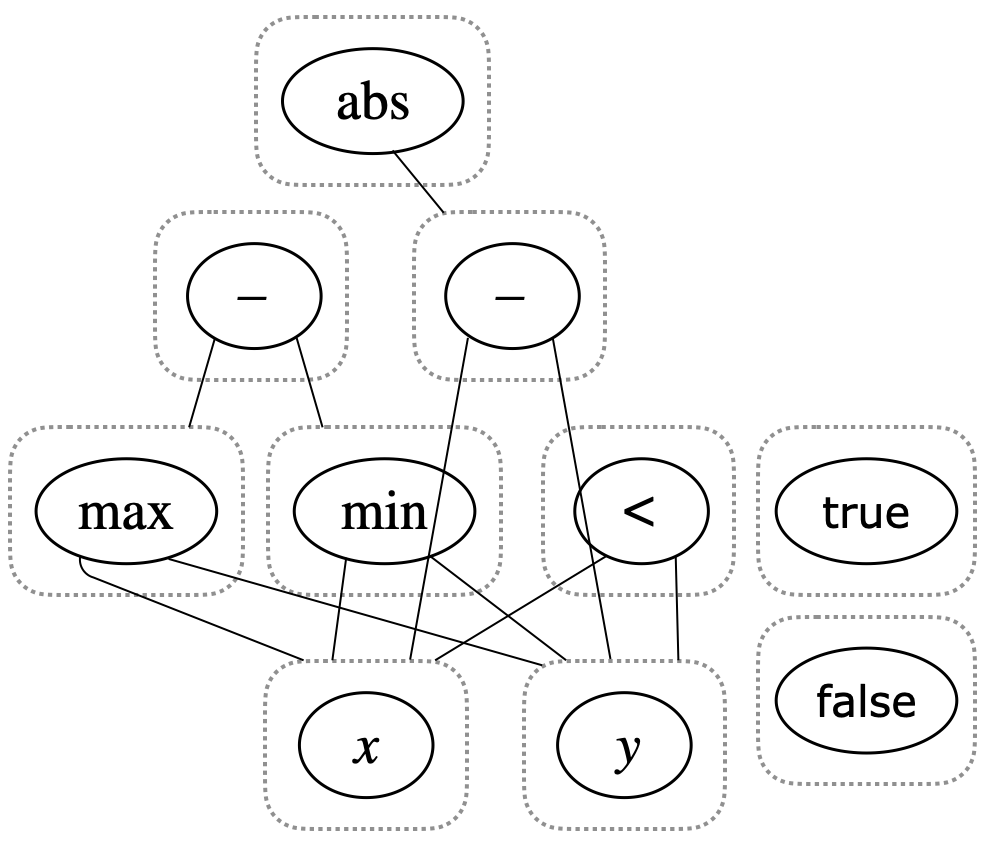
\includegraphics[width=0.25\textwidth]{colors/gfx/egraph-max-min.png} &
    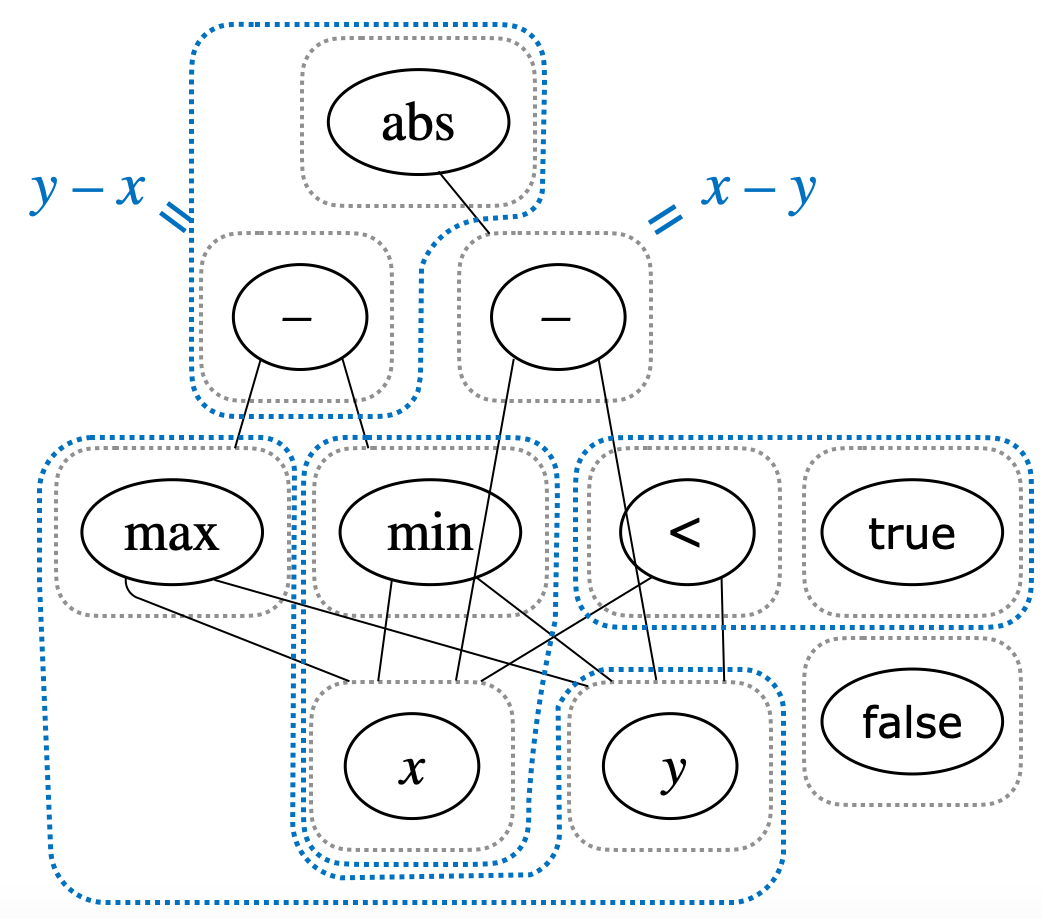
\includegraphics[width=0.25\textwidth]{colors/gfx/egraph-max-min-blue.png} &
    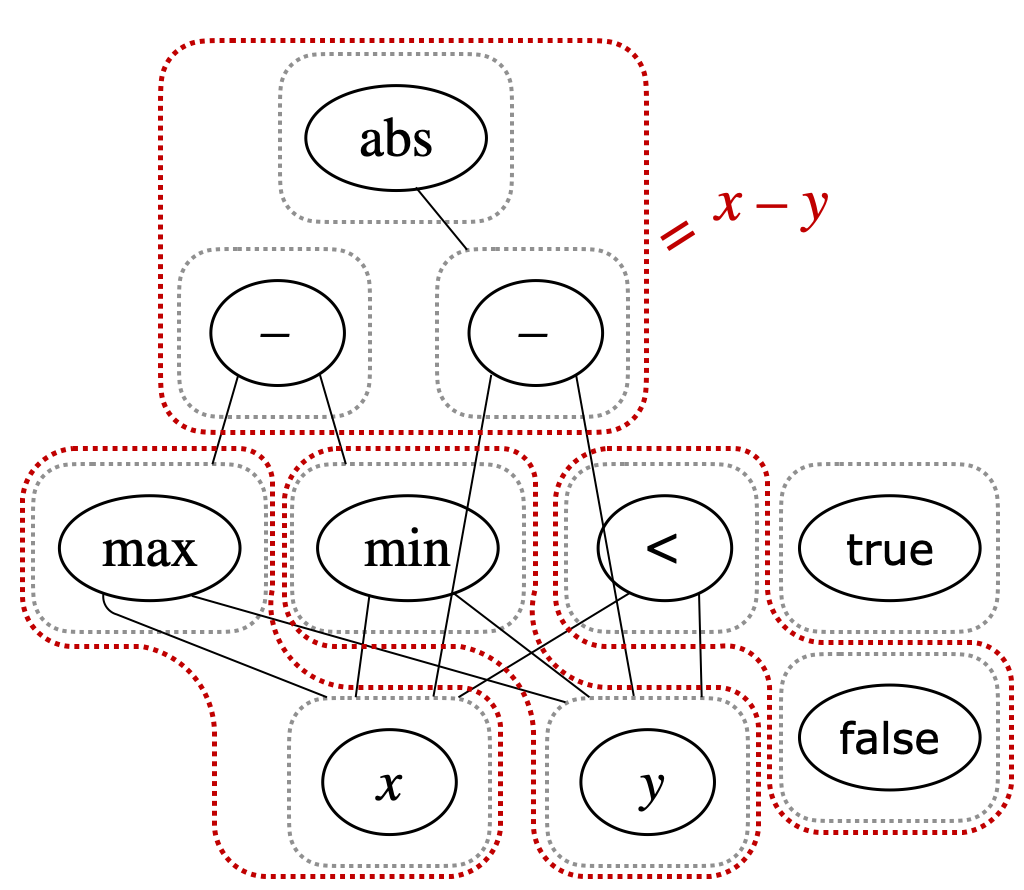
\includegraphics[width=0.25\textwidth]{colors/gfx/egraph-max-min-red.png}
    \\
    {\small (a)} & {\small (b)} & {\small (c)}
  \end{tabular}
  \caption{Proof of $\tsmallmax(x,y)-\tsmallmin(x,y)=|x-y|$.
  The e-nodes corresponding to the two terms are in the same e-class both in the blue layer (b) and in the red (c).
   It is important to note that the layers are overlain, and that the black nodes are shared; they are separated here for ease of perception.}
  \label{overview:egraph-max-min}
\end{figure*}

Both additional layers, \cblue and \cred, use existing (black) e-nodes, with each color represented by further unions of e-classes in the black congruence relation. 
Each color's congruence $\cong_c$ is a \emph{coarsening} of the black congruence, $\cong$, as ${\cong}\subseteq{\cong_c}$.
% Hierarchy exmaple
In complex cases like the generalization of $\tmax(x,y)-\tmin(x,y) \cong |x-y|$ to $\tmax(x,y,z)-\tmin(x,y,z) \cong \tmax(|x-y|, |x-z|, |y-z|)$, the colored e-graphs have an important layered structure. 
This scenario requires reasoning about additional assumptions, building additional layers, such as $x < y \land y < z$ on top of $x < y$ (and respectively $x \ge y \land y < z$ on top of $x \ge y$). 
These additional layers will reuse the \cblue and \cred ones, as they are a coarsening of the respective $\congblue$ and $\congred$.

\begin{comment}
The extra colors are due to the conditionals from $\tmax$, $\tmin$, and $|\,{\cdot}\,|$ leading to a total of six leaf cases as can be seen in \autoref{overview:minmax-splits}.
The coarsening of congruence relation holds in this multi-level hierarchy as well.
If we mark in \cblue the layer representing $(x < y) \congblue \ttrue$, and in \cgreen the layer representing $x < y \land y < z \conggreen \ttrue$, then ${\congblue}\subseteq{\conggreen}$.
That is, any common sub-term and conclusion made in root, or one of the parent colors can be shared to the descendants.
Thus, further duplication, whether of terms or computation, can be prevented.
%Note, that this is not a full tree as in some cases we can conclude the $<$ relation between $x$ and $z$. 
%For example, in the case of $x < y \land y < z$ we can conclude $x < z$ without additional case splitting.

\begin{figure}
\begin{tikzpicture}[
    grow=down,
    level 1/.style={sibling distance=50mm, level distance=20mm},
    level 2/.style={sibling distance=25mm, level distance=20mm},
    level 3/.style={sibling distance=25mm, level distance=20mm},
    edge from parent/.style={->, draw},
    >=latex,
    every node/.style={align=center}]

% root of the tree
\node (root) {root}
% children of root
    child{node {$x < y$}
        % children of "x >= y"
        child{node {$x < y \land y \ge z$}
            child{node {$\cdots \land x < z$}}
            child{node {$\cdots \land x \ge z$}}
        }
        child{node {$x < y \land y < z$}}
    }
    child{node {$x \ge y$}
        % children of "x < y"
        child{node {$x \ge y \land y \ge z$}}
        child{node {$x \ge y \land y < z$}
            child{node {$\cdots \land x < z$}}
            child{node {$\cdots \land x \ge z$}}
        }
    };
\end{tikzpicture}
\caption{All needed case split cases to reason about the property $\tmax(x,y,z)-\tmin(x,y,z) \cong \tmax(|x-y|, |x-z|, |y-z|)$}
\label{overview:minmax-splits}
\end{figure}
\end{comment}

\begin{comment}
A crucial challenge to address is the implementation of operations (insert, union, congruence closure, e-matching)
efficiently while preserving this invariant as well as the standard e-graph invariants.
The colored layers require special support, as different e-classes may be united in some colored (non-black) layer but not in others (including the black relation). 
Notably, the black congruence relation can be implemented as a standard e-graph since all the necessary data structures are available to it.
\end{comment}

% Clone semantics
Before diving into the design of colored e-graphs, it is better to start with their expected semantics.
One way to understand the semantics of colored e-graphs is by analogy to a set of clones, i.e. separate e-graphs $\mathcal{E}$.
One e-graph represents the base congruence $\cong$,
and one e-graph per color $c$ represents $\cong_c$.
All e-graphs in $\mathcal{E}$ conceptually represent the same terms partitioned differently into e-classes.
Thus, they have the same e-nodes, except that the choice of e-class id (the representative) may be different according to the composition of the e-classes.
We will call the e-classes of the color congruences \emph{colored e-classes}.
A union in any layer, black or colored, is in effect a union applied to the respective e-graph and all its descendants. 
Thus, a union in the black layer (i.e. the original e-graph) is analogous to a union in \emph{all} of the e-graphs of the corresponding e-classes;
this maintains the invariant that every colored e-class is a union of (one or more) black e-classes.
The colored e-graph semantics of the other operations---insertion, congruence closure, and e-matching---are the same as if they were performed across all clones.

\begin{comment}
Using a set of e-graphs is very similar to what TheSy does.
But, this set of e-graphs approach proves to be inefficient in exploratory reasoning tasks. 
The main issue is that with each e-graph consisting of its own hash-cons, union-find, and e-class map, the memory consumption will be significant.
However, in some cases a separate e-graph could be quite efficient.
An extreme (but not uncommon) case is when an e-graph becomes inconsistent, which can be when \eg $\ttrue$ is union-ed with $\tfalse$.
This can lead to many e-classes representing Boolean expressions being union-ed, and as a side effect, requiring much fewer e-nodes.
For example $\ttrue \land \ttrue$, $\ttrue \land \tfalse$, $\tfalse \land \ttrue$, and $\tfalse \land \tfalse$ will all be represented by the same e-node $[\ttrue] \land [\ttrue]$.
In this case, when the e-graph rebuilds it will minimize itself.
The e-graph memory footprint could actually be as small as the size of the union-find plus a constant amount of e-nodes.\SI{I am a bit unsure about how `constant' this amount is; still sounds polynomial in the number of e-classes}
\end{comment}

A guiding observation in the design is that in equality saturation based exploratory reasoning tasks, where the e-graphs are extensive, each assumption leads to modest increase in congruences.
Colored e-graphs are adapted to this scenario.
The basic presupposition is that most colored layers, like the \cblue layer in \autoref{overview:egraph-max-min}, do not involve an excessive amount of additional unions.
In these cases, the space savings from not duplicating black e-nodes more than compensate for the added complexity in managing colored e-classes. 
With careful tweaks and a few optimizations, we show that we improve upon a clone-based approach.
Importantly, if the assumption leads to an inordinate increase in additional unions, the clone-based approach could be more appropriate, and it is possible to use a clone for that specific assumption.

%\SI{there is some commented-out content here}
\begin{comment}
%As we will show later, the colored e-graph performs worse when many changes are done on top of the original e-graph \ES{TODO: show and link?}.
And so, colored e-graphs and separate e-graphs are approaches that complement each other.
An obvious optimization is to automatically switch from a colored layer into a new separate e-graph on the fly.
This can potentially improve performance, but automatically detecting when it is useful, and then switching is something we leave for future work. 
\ES{TODO: we need to make sure we right about the inherent problems in the colored e-graph implementation when there are many changes (after the optimizations). then add this but with more detail: Although it might seems like a limitation, but actually we can always decide to drop a color, or explore it in a new separate E-Graph.}
\end{comment}

% The most basic setup. Without colored e-nodes, only how we implement rebuild and e-mathcing.
For presentation purposes, we start with a basic implementation that is not very efficient but is effective for understanding the concepts and data structures;
then, we indicate some pain points, and move on to describe optimization steps that can alleviate them.

In the basic implementation, all e-nodes reside in the ``black'' layer,  represented by a ``vanilla'' e-graph implemented in egg, with normal operations.
The colored congruences do not have designated e-graphs of their own, and instead, the operations of merge, rebuild, and e-matching have \emph{colored variants}, parameterized by an additional color $c$, that are semantically analogous to the same operations having been applied, in clone semantics, to the e-graph associated with color $c$ in $\mathcal{E}$.
(Insertion is deferred to later.)
%(For the time being, insertion does not have a colored variant, since insertions create e-nodes and all e-nodes are shared.)

\myparagraph{Colored merge.}
In colored e-graphs, the union-find structure used for merging, which traditionally holds all e-class ids, is optimized. 
A master copy retains black unions, while each color layer has a \emph{smaller} union-find for merged representative e-classes of the parent layer. 
This approach avoids replication of data across layers.

\myparagraph{Colored e-matching.}
The e-class map is only saved for the black layer.
This is sufficient, because an e-class in color $c$ is always going to be a union of black e-classes, and all that is required for e-matching is finding e-nodes with a particular root (operator) in the course of the top-down traversal.
So the union can be searched on demand by collecting all the ``$c$-color siblings'' of the e-class and searching them as well.

\myparagraph{Colored congruence closure.}
In egg, the e-graph maintains congruence by cycling through a work list of altered classes, re-canonizing their parents, and identifying unions to complete congruence through duplicate detection.
In colored e-graphs the root will behave the same, but for colored layers there is no single e-class, as the colored e-classes are a equality class of concrete e-classes.
For each color, we maintain an additional work list and collect concrete parents from e-classes on demand. 
This results in a rebuild algorithm similar to egg's, but without updating the hashcons in colored layers, as they are not present.

For a more concrete example, we give a detailed walkthrough of equality saturation in a colored e-graph of the \cred case from  \autoref{overview:egraph-max-min}(b), and show the steps taken
to construct this colored layer in \annexref{app-b}.

When using the above operations in the context of equality saturation, e-matching is applied for all colors
% \SI{should we describe the machine way to do it in a combined pass or leave it for optimizations} - Leave for optimizations. It is a non trivial optimization to say black matches cover colored ones. 
to discover matches for the left-hand sides of rules.
For each match, the right-hand side of the rule needs to be inserted into the e-graph and merged or color-merged with the left-hand side.
Inserting the e-nodes to the e-graphs makes them available to all layers.
This aspect is sound, since
we assume that the mere \emph{existence} of a term in an e-graph does not in itself have the semantics of a judgement---it is only the placing e-nodes in the same e-class that asserts an equality.
However, in the presence of many colors, and thus many colored matches, the result would be a large volume of e-nodes that are in black e-classes of size 1, as they
were created to serve a single color.
As opposed to a, standard, single e-graph where merging e-classes shrinks the space of e-nodes (because non-equal e-nodes may become equal as a result of canonization),
in colored unions it is required that the e-graph maintain both original e-classes, thus losing this advantage.
This can put a growing pressure on subsequent e-matching and rebuild operations \emph{in all colors}.
Optimizations to improve colored e-graphs, and to address this issue, are presented in \autoref{colors:optimizations}.


\begin{comment}
   {\color{gray} 
\noindent\textbf{Colored insert.}~
As discussed, e-nodes should be shared, but until now no new e-nodes were added.
A simple example is the e-graph for the terms $1 + 2$, $2 + 1$ and $x$.
Now consider a new {\color{blue}blue} relation, and have the blue union $1 \congblue x$.
When we apply addition commutativity on this e-graph, a new e-node, ($1~+~x \rightarrow x~+~1$), should be added, but only for the blue layer.
In the current unoptimized approach, we share all e-nodes, so there will only be black e-nodes.
Meaning we will add the e-node to the original e-graph, but only unify the e-classes in the blue layer.
\ES{Should this be a theorem?} It is sound under the assumption that any e-node in the e-graph does not have any semantic meaning by itself.
For example, when encoding a problem to the colored e-graph, $sorted(l)$ has no semantic meaning unless $sorted(l) \cong true$ or $sorted(l) \cong false$.
And, If an additional e-node represented in the original e-graph does not affect the semantics, it is safe to add all colored conclusions as black e-nodes.


% Caveats and intro to optimizations section
To understand the weakness of this simple approach we should consider the setting of equality saturation.
A color will have additional unions, and therefore, might apply more rewrites resulting in additional e-nodes. 
The most basic approach of adding these e-nodes to the existing e-classes, hash-cons, and parents, is sound, but will result in additional e-matching results.
When considering the example from before, all colors can match on $x~+~1$.
A larger e-graph with more e-matches will lead to more rewrite rules being applied, and a slower rebuild process.
In addition, colored e-matching can find colored un-canonized matches.
Canonizing matches using the black congruence relation may lead to the addition of many unneeded e-nodes, as colored e-matching might produce duplicate matches.
But, canonizing using the colored congruence relation might produce different e-nodes for each color.
What makes matters more difficult, is that when all e-nodes are part of the original e-graph, they will not remain canonized by the colored relation, and might become "dangling" \ES{We will need to work on these explanations}.
}
\end{comment}

\section{Functional Description}
\label{colors:functional}

We now introduce some notations and definitions that formalize
the description of the e-graph presented in \autoref{colors:overview}.
We assume a term language $L$ where terms are constructed using \emph{function symbols}, each with its designated arity.
We use $f^{(r)}\in\Sigma[L]$ to say that $f$ is
in the \emph{signature} of $L$ and has arity $r$.
A term is then a \emph{tree} whose nodes are labeled by function symbols and a node labeled by $f$ has $r$ children.
(In particular, the leaves of a term have nullary function symbols.)
Additionally we use the following definitions:
%
\[
\renewcommand\arraystretch{1.2}
\begin{array}{ll}
  \mbox{e-class ids} & E  \\
  \mbox{e-nodes}  & N = \{f(e_1,..,e_r)~|~ f^r\in\Sigma, e_i\in E\} \\
  \mbox{union-find} & {\eqid} \subseteq E\times E, \quad \mbox{${\eqid}$ is an equivalence relation} \\
  \mbox{e-class map} & M : E \to \mathcal{P}(N) \\
  \mbox{parent map}  & P = \{e \mapsto \{ (n, e') ~|~ e' \in E~\land \\
  & \quad n \in M(e') \land n = f(\ldots, e, \ldots) \} ~|~ e \in E \} \\
  \mbox{hashcons} & H = \{n\mapsto e ~|~ n\in M(e)\} \\
\end{array}
\]

Semantically, every e-class represents a set of terms over $\Sigma$.
We will use the notation $[t]$ to refer to e-class id of the equality class that represents (among other terms), the term $t$.

The union-find structure offers an operation, $\tfind(e)$, that returns a unique representative id of the equivalence class (of $\eqid$) that contains $e$.
That is, $\tfind(e) \eqid e$ and for all $e_1 \eqid e_2$, $\tfind(e_1) = \tfind(e_2)$.

On top of these basic structures, we introduce a set of \emph{colors}. 
As explained in \autoref{colors:overview}, colors are organized in a tree whose root is the initial color (``black'').
We mark the root color $\croot$
and assign to every non-root color $c$ a \emph{parent color} $p(c)$.
%
\begin{comment}
\[
\begin{array}{ll@{~~~}l}
\mbox{color tree} & C = \{\croot, \ldots\}
& p : C \setminus \{\croot\} \to C
\end{array}
\]
\end{comment}
\[
\renewcommand\arraystretch{1.2}
\begin{array}{ll}
  \mbox{colors} & C = \{\croot, \ldots\}  \\
  \mbox{parent colors} & p : C \setminus \{\croot\} \to C
\end{array}\hspace{2cm}
\]

\smallskip
The colored e-graph will now hold multiple union-find structures, one per color.
They define a family of equivalence relations $\equiv_{c}$ by induction
on the path from $\croot$ to $c$.

\begin{itemize}
    \item ${\equiv_{\varnothing}} = {\eqid}$~;\quad $\tfind_{\varnothing}(e) = \tfind(e)$
    \item ${\equiv_c} \subseteq E_{p(c)}\times E_{p(c)}$, where
      $E_{p(c)}=\{\tfind_{p(c)}(e)~|~e\in E\}$ is the set of all representatives from $\equiv_{p(c)}$. $\tfind_c\hspace{-0.5pt}(e)$ for $e\in E_{p(c)}$ returns a unique identifier in the normal manner of union-find, \ie, $\tfind_c\hspace{-0.5pt}(e) \equiv_c e$  and for all $e_1 \equiv_c e_2$, $\tfind_c\hspace{-0.5pt}(e_1) = \tfind_c\hspace{-0.5pt}(e_2)$.
\end{itemize}


\begin{comment}
Formalize the colored-rebuild algorithm
This should include an algorithmic description of normal rebuild
Then we would use functions to use the same algorithm for colored rebuild.
The main concerns that change are:
1. Collecting all the parents
2. Updating the memo
\end{comment}

The definitions over $E_{p(c)}$ are naturally extended to $E$ by (recursive) application of $\tfind$; i.e., $\tfind_c(e) = \tfind_c(\tfind_{p(c)}(e))$
and $e_1 \equiv_c e_2 \Leftrightarrow \tfind_{p(c)}(e_1) \equiv_c \tfind_{p(c)}(e_2)$.
Thus it holds, by construction, that
${\equiv_{c}} \supseteq {\equiv_{p(c)}}$.

The colored e-graph also supports a $\tmerge_c(e_1, e_2)$ operation for each color $c$ where $e_1, e_2 \in E_c$.
The merge operation may break the congruence relation invariants for $c$ and all its descendants, and thus needs to be fixed.
The merged classes are added to $\mathit{worklist}(c')$ for all $c'$ where $c'$ is $c$ or one of its descendant.
In egg~\cite{egg}, the invariants are restored periodically by performing a \textsc{rebuild} pass.
To accommodate the colors, we adjust the
\textsc{rebuild} logic to a multi-congruence-relation setting,
so that it restores a congruence closure for each color during \textsc{rebuild}.
The main difference is that for a colored congruence relation, the procedure will collect the parents of a colored e-class by combining the sets of parents of all the (root) e-classes contained therein.

\begin{comment}
We update the auxiliary function \textsc{repair}
to work on colored e-classes,
and introduce two new helper functions: $\textsc{collect\_parents}$ and $\textsc{update\_hashcons}$, as presented in \autoref{functional:repair}.
$\textsc{collect\_parents}$ extract the parents of a colored e-class by combining the sets of parents of all the (root) e-classes contained therein.
$\textsc{update\_hashcons}$ is used to make sure that the hashcons entries are in canonical forms. It was already a part of \textsc{repair} in egg;
it is only repeated here to point out that it
only updates the hashcons for the root color,
since no canonization is required for colored layers.    
\end{comment}

Another important colored e-graph operation is e-matching.
Colored e-matching is a modification of the e-matching abstract machine presented in \cite{DBLP:conf/cade/MouraB07}.
E-matching is performed by an abstract machine $M$ which consists of a program counter, array of registers $reg$, and backtracking stack $bs$, in combination with a sequence of instructions that represents a pattern $p$. 
The machine will run instructions by order, where each may either fail if its assertion is not met, or produce a set of continuation states.
If a continuation state is produced, the machine selects the first one and adds the current instruction to the stack. 
If no continuation state is produced, the machine backtracks, retrieving the most recent state from the stack and attempting the next available continuation.

To better present our modifications in colored egg, we first shortly introduce some of the original instruction types:
\begin{itemize}[leftmargin=1.1em]
    %\item $\iinit(f)$ --- Expects an e-node representing an application $f(x_1,\ldots,x_n)$ in $\treg[0]$, and pushes its children into $reg[1..n]$.
    \item $\ibind(\tin, f, \tout)$ --- Matches any e-node of the form $f(x_1,\ldots,x_n)$ that resides in the e-class saved in $reg[in]$, storing its children $x_{1..n}$ in $reg[out..out+n-1]$.
    \item $\icompare(i, j)$ --- Asserts $\treg[i] == \treg[j]$.
    \item $\icheck(i, term)$ --- Asserts that the e-class $\treg[i]$ represents $\tterm$.
    \item $\icontinue(f, out)$ --- Match any e-node 
    $f(x_1,\ldots,x_n)$ (in \emph{any} e-class),
    storing its children $x_{1..n}$ in $\treg[\tout..\tout+n-1]$.
    \item $\ijoin(\tin, \trevpath, \tout)$ --- Match any e-node
    $f(x_1,\ldots,x_n)$ that is reachable through $\trevpath$
    from the e-class $\treg[\tin]$,
    storing its children $x_{1..n}$ in $\treg[\tout..\tout+n-1]$.
\end{itemize}

To facilitate matching across various congruence relations, we adjust the machine $M$ to include the, currently being e-matched, colored assumption $color$ in its state.
Adapting to $color$ involves changes in compilation and instructions. 
The two primary scenarios impacted are: during $\icompare(i, j)$, ensuring $\treg[i] \equiv_{color} \treg[j]$, and in function application matching represented by a \ibind~ instruction.
Before each `\ibind' instruction, the modified compilation will insert a new `\iclrjmp' instruction to try matching the full colored equality class, one ``root'' e-class at a time.
This is achieved by having `$\iclrjmp(i)$' yield all the ``colored siblings'' of $\treg[i]$ in the current $\tcolor$, replacing $\treg[i]$ with the result.
%The algorithms for \textsc{colored\_jump}($i$) and the updated \textsc{compare}($i, j$) are given in \autoref{functional:colored_machine}.
The instruction `check' can be likewise adjusted, but we point out
that, in fact, it can be implemented as a sequence of `\ibind's (with respective interleaved `\iclrjmp's).

Multipatterns, supported by the abstract machine, enable e-matching against patterns with shared variables, useful for matching the precondition in conditional rewrite rules.
This is achieved using the `\icontinue' instruction, which selects a new root for subsequent sub-patterns. 
In the colored setting, while `\icontinue' remains as is, for performance, it's sometimes substituted with `\ijoin'. 
This alternative instruction also picks a new root, but restricts selection to e-nodes that can reach a specified e-class, linked to a previously matched hole, through child edges in the e-graph.
A \emph{reverse path} is provided to further restrict the upward search needed to find such e-nodes.
We do not go too deep into the details, but its colored variant
will invoke a $\iclrjmp$ at every level.
We point out that egg does not currently implement `\ijoin',
and our colored egg supports a special (though frequent) case in which
$\trevpath$ is empty.

The algorithms described here are presented in more depth in \annexref{app:algorithms}.
\section{Optimizations}
\label{colors:optimizations}

% How we should present this section:
%
%   Intro
%   Show problems that are existing still:
%       a. go into the just presented bad rebuild - go into the e-node count
%       b. inform on worse ematching with duplicate results
%       c. e-node readding
%   sub-section 1 data structure
%   2. Improve data structure to somewhat reduce these problems - Represent colored e-nodes seperately
%       a. Assume small changes again
%       Also Deals with previously presented problems:
%       b. We have a canonized version of colored conclusions to somewhat prevent readding.
%       c. No extra results in e-matching because of seperation.
%       d. Might want to go into big changes complements clones
%   3. We can prune unneeded e-classes in an attempt to improve memory usage for long runs (probably more relevant in cases where some rewrite rules will be used less, to prevent readding).
%   4. A small optimization of having one colored e-class per colored equality class
%   sub-section 2 algorithms
%   Algoritmic improvements that can be made without changes to data structures.
%   5. Improve e-matching by reusing black results as black
%       a. We jump to brothers only on a different "black" path to prevent duplicate paths in the e-graph
%       b. Might be harder to apply conditions
%   6. Improve rebuilding by reusing black conclusions
%   subsection 3 system upgrades
%   As part of the change to colored e-graphs, some other parts of the system might need to change
%   7. e-matching should stream results as we e-match all colors at once
%   8. condition checking needs to actively check all colors for black matches

% Stuff we did not do:
%   1. Parallel colored congruence
%   2. Hierarchical colors
%   3. Had the possibilty of coloring only e-nodes, but that makes the rebuilding process very difficult

\begin{comment}
This section details key optimizations for colored e-graphs, addressing challenges encountered when applying operations such as e-matching and rebuilding.
These optimizations target issues like handling e-nodes across multiple layers, inefficient rebuild processes, duplicate results in e-matching, and e-node re-additions. 
We'll first outline these issues before presenting solutions.    
\end{comment}

Both rebuilding and e-matching in colored e-graph, as discussed in \autoref{colors:overview}, can be significantly slower compared to a separate, minimized e-graph.

In the rebuilding aspect,
two main burdens are that the colored e-graph contains additional e-nodes compared to each of the separate ones, and that building a colored hash-cons (which will be presented shortly) requires going over all the e-classes.

In the e-matching aspect, colored e-matching
may produce duplicate results due to the e-graph not being minimized according to the color's congruence relation;
that is, colored-congruent terms are not always merged under a single e-class id.
To illustrate this, consider a simple e-graph
representing the terms $1\cdot 1$, $1\cdot x$, $1\cdot y$, and $x\cdot y$.
Introduce a color, \cblue, where $x \congblue y$.
A simple pattern such as $1\cdot ?v$ would have three matches, with assignments $?v \mapsto 1, ?v\mapsto x, ?v\mapsto y$.
If the \cblue layer were a separate e-graph, $x$ and $y$ would have been in the same e-class,
so one of the matches here is redundant (as far as the blue layer is concerned).
Of course, in the black layer they are different matches; the point is, that many terms are added to the graph only as a result of a colored match,
so matching them in the black e-graph is mostly useless to the reasoner.
On the other hand, their \emph{presence} in the black layer means they cannot ever be merged, leading to duplicate matches, as seen above, even in the respective colored layer(s).

Moreover, when inserting e-nodes to the e-graph, the hash\-cons is used to prevent duplication, relying on it being canonized.
Adding an e-node from a colored conclusion
(following a match modulo $\congbluesym$) does not benefit from canonization.
In fact, each e-node $f(x_1,\dots,x_n)$ has a multitude of black representatives that are $\congbluesym$-equivalent. 
Each child $x_i$ in the e-node can be presented by any black id such that $e \in [x_i]_b$, so there are $\prod_i |[x_i]_b|$ representations.
These variants are distinct in the root color,
so they cannot be de-duplicated as usual.

To address these issues, we present a series of optimizations to the colored e-graph data-structure and the procedures. 
These optimizations aim to reuse the ``root'' and ancestor layers as much as possible, both in terms of memory usage and compute.
Thus, we can achieve a memory efficient, but effective colored e-graph. 

\subsection{Data-structure optimizations}
% Having the seperate differences
\myparagraph{Colored e-nodes.}
In the basic implementation outlined in \autoref{colors:overview}, adding e-nodes from colored e-matches to the root e-graph may make it very large and increase the cost of all subsequent actions. 
The optimized version addresses this by introducing \emph{colored e-nodes}, where e-nodes resulting from colored matches are tagged with their inducing colors. 
Each colored layer has its own colored hash-cons and e-class map, designed to store only the differences from the parent layer, thereby maximizing reuse.
The new mappings added are:
%\newcommand\eqid{\equiv_{\mathrm{id}}}
%
\[
\renewcommand\arraystretch{1.2}
\begin{array}{ll}
  \mbox{e-class color}& \! \! EC : E \to C  \\
  \mbox{colored parent}& \! \! P_c = \{ (n, e) ~|~ (n, e) \in P \land EC(e) = c \} \\
  \mbox{colored hashcons}& \! \! H_c = \{n \mapsto e ~|~ n \in M(e) \land EC(e) = c \} \\
\end{array}
\]

Note that base parents and hashcons from the non-optimized version are incorporated as $P_\croot$ and $H_\croot$ in colored mappings.

This optimization applies the hierarchy in all operations. 
For example, while inserting an e-node to a color $c$, it is looked up in the colored hash\-cons for $c$ and all its ancestors, $p^*\!(c)$, and finally, if no match is found, it is inserted into a new e-class $e$, setting $EC(e) = c$.
The colored hashcons $H_c$ is canonized to color $c$, ensuring that new e-nodes are unique to this layer and avoiding colored duplicates. 
(Some duplication related to $c$ may still occur in ancestor layers, as their e-nodes are not canonized to $c$.)
The optimization significantly impacts e-matching: previously when matching a function application $f$, all $f$-e-nodes in $N$ were considered; now, only those e-nodes $n$ in the colors hierarchy, that is, those satisfying $\exists e.~n \in M(e) \land EC(e) \in p^*(c)$, are examined.

% Assume small changes
%\SI{why is this paragraph in this particular place}
%The optimized version of the colored e-graphs will have additional e-nodes for each color.
%In the context of equality saturation, any additional colored e-node results from some rewriting conclusion, so the more colored unions happened, the bigger we expect the colored e-graph to be, tying the size of the colored e-graph to the, assumed to be small, changes introduced under each color.

% Present pruning
\myparagraph{Pruning.}
Recall that having a coarsening relation between the colors in the hierarchy means that any result found in an ancestor color is also true for the descendant(s).
And so, following merges, some of the colored e-nodes could become subsumed by e-nodes that already exist in an ancestor layer.
We present an efficient deferred pruning method to remove the redundant e-nodes.

Normal e-graph minimization relies on having all e-nodes canonized.
A colored e-graph usually does not canonize all e-nodes to a specific color $c$ (except for \croot). 
Rather, $H_c$ contains only the difference from previous layers. 
To find redundant e-nodes, the colored e-graph  builds a transient hashcons during rebuild from all relevant e-nodes that are not $c$-colored.
The new hashcons, $H'_c$, is created as follows:
\[
\renewcommand\arraystretch{1.2}
\begin{array}{l@{}l}
H'_c = \{& \mathit{canonize}_c(n) \mapsto \tfind_c(e) ~|~ \\
& ~~n \in M(e), EC(e) \in p^+(c) \}
\end{array}
\]
% redundant = $\{ n | \exists e. n \in M(e) \land EC(e) = c \land n \in H'_c \}$
A $c$-colored class $e$ can be reduced by removing all e-nodes that already exist in $H'_c$.
While pruning is promising, one must take care that pruned e-nodes are not immediately re-added.
% We can add that this is probably when we add conclusions back to the black layer or we stop using certain rewrite rules.

% Present the "single colored e-class per colroed equality class" thing
\myparagraph{Colored minimization.}
Another improvement is having multiple colored e-nodes (of the same color) in a single (black) e-class. 
As mentioned previously, any e-node that resulted from a colored insert had to be in their own e-classes, as no black unions would be performed on them.
But, given that $e \equiv_c e' \land EC(e) = EC(e') = c$, then the two black e-classes $e,~e'$ can be merged as both contain colored e-nodes of the same color and are in the same colored e-class (of the same color).
Thus an invariant is kept that each colored equality class has at most one black e-class containing colored e-nodes.

\subsection{Procedure optimizations}
%   6. Improve rebuilding by reusing black conclusions
\myparagraph{Rebuild.}
When rebuilding, we first reconstruct the congruence relation of the ``root'' layer.
Even though a color, for example {\color{blue}blue}, will need to rebuild its own congruence, it still holds that ${\cong}\subseteq{\congblue}$.
So, any union induced by ${\cong}$ can be applied to the {\color{blue}blue} relation.
To understand the implications, consider the e-graph representing the terms $x$, $y$, $f(x)$, $f(y)$, $f(f(x))$, and $f(g(y))$ where the {\color{blue}blue} color contains the additional assumption that $g(y) \congblue f(y)$.
If we union $x$ and $y$, the black congruence will include $f(x) \cong f(y)$  which also holds in the blue relation.
But, the rebuilding of the blue congruence invariant will include an additional, deeper (in terms of rebuilding rounds), conclusion $f(f(x)) \congblue f(g(y))$.
This demonstrates how reusing parent relations is useful; the rebuild depth can be reduced by first rebuilding finer relations.

%   5. Improve e-matching by reusing black results as black
%       a. We jump to brothers only on a different "black" path to prevent duplicate paths in the e-graph
\myparagraph{E-match.}
In e-matching, we implement an optimization where findings on the root layer are also valid for higher layers. 
To avoid redundant pattern matching, e-matching begins only from \croot, adding colored assumptions as needed. 
There are two scenarios for introducing a colored assumption: 
The first during \emph{compare($i, j$)}, if $\treg[i] \not \equiv_{\tcolor} \treg[j]$, we explore descendant colors $c$ where $\treg[i] \equiv_c \treg[j]$, adding states with $\tcolor \gets c$ to the backtracking stack $bs$.
The second is on-demand coloring in \iclrjmp, where jumps to any color $c$ are enabled if $M.color \in p^+(c)$ and the target e-class is otherwise unreachable.
We minimize the set of new assumptions to prevent redundant colors. 
During the updated \icompare, \icompare', if a color $c$ is sufficient, its descendants are not added to $bs$. 
For to updated \iclrjmp, \iclrjmp', e-classes are matched only with their topmost (closest to root) congruent descendants. 
By taking the topmost descendants, we ensure that all additional matching paths are unique, as at least one (different) e-class is chosen at each fork.
Despite eliminating duplicate paths, some duplicate colored matches persist due to incomplete minimization of the e-graph.
The modified instructions are described in more detail in \annexref{app:algorithms}. 

\begin{comment}
    To support matching multiple colors at once, we modify the machine such that it will add colored assumptions on demand during the search, and push it into the backtracking stack $bs$.
    For that purpose, we modify $M$ to also include the current colored assumption $color$, which will be initialized to $\varnothing$.
    There are two situations where a colored assumption will be added.
    The first is during \emph{compare($i, j$)}.
    If $reg[i] \neq reg[j]$, then we don't necessarily need to backtrack, as there might be a descendant of $color$, $c$, under which $reg[i] \equiv_c reg[j]$.
    Therefore, for each such $c$ the current state with the new assumption $color \gets c$ is add to the backtracking stack $bs$.
    The second case is when matching a function application of $p$ which is represented by a bind instruction.
    Before each bind instruction, a modified compilation procedure will insert a new \emph{colored\_jump} instruction.
    The \emph{colored\_jump($i$)} instruction will add all the "colored siblings" of the current $color$ to $bs$.
    In addition any additional colored assumption $color`$ that is descendant of $color$, and has additional "colored siblings" will also be pushed to $bs$.
    The algorithms for \emph{colored\_jump($i$)} and the updated \emph{compare($i, j$)} are given in \ES{TODO}.
\end{comment}


%       b. Might be harder to apply conditions

%  TODO: I think we should not include system upgrades.
% subsection 3 system upgrades
%   As part of the change to colored e-graphs, some other parts of the system might need to change
%   7. e-matching should stream results as we e-match all colors at once
%   8. condition checking needs to actively check all colors for black matches



% Therefore, TheSy does not keep all the assumptions (E-Graph clones). Rather, TheSy uses the case splitting mechanism to find relevant equalities only at a few strategic points in the exploration, and then frees all the clones to save memory.
% \ES{smoother}
% We aim to further amortize costs while enhancing the memory usage efficiency of the E-Graph, by maximizing component reuse. 
% This approach requires a detailed understanding of the primary data structures employed by the egg library. 

% Remind use case and go over the problems we need to deal with when no colored e-nodes
\begin{comment}
Colored e-graphs are designed to be used in larger scale test cases where some tool is using the e-graph for exploration tasks.
This means that the e-graph will contain numerous e-nodes, and possibly multiple colors.
While we hope the reader is convinced our e-node sharing approach is useful, the solution provided so far will be inapplicable to any real case.
The main culprit is that we insert all e-nodes to the black relation.
Having all e-nodes exists in the black relation means they will also exist for all colored relations.
While this doesn't seem detrimental to the performance at first, the problem actually arises from having additional successful applications of rewrites.
Of course it seems like a good thing because each application retains soundness, and we gain more conclusions in the e-graph.
But, having all these conclusions means that even for each additional e-node we might attempt to match it in additional rewrites, and the rebuilding will need to go over it.
Also, rebuilding for colored congruence relations, which is inefficient, will need to be applied to all e-nodes of all colors.
\end{comment}

% A good example: For optimizations: For example, in a relation where all E-Classes are unioned, E-Matching will be very inefficient due to the caveat we presented.
% This issue becomes more pronounced when considering the additional results in e-matching. As the number of successful rewrite applications increases, more e-nodes are added to the e-graph. This may seem beneficial, as each application maintains soundness and results in more conclusions within the e-graph. However, in our experiments [TODO], we do not observe any of these advantages.


\section{Evaluation}
\label{colors:eval}

% Why and what we want to check
% How we are going to check
% Where we check it - i.e. computer

% Experimental setup:
% 1. Memory cap + stats using Cap
% 2. Using problems from cvc4 induction with aggregated proof terms
% 3. Configurations - runtime, memory 
% Problems in creating an experiment with existing systems
% Different variants being tested and implementations. Everything is based on TheSy's case split mechanism.
% 1. TheSy cloning, but keep splits to simulate memory use
% 2. TheSy with colors - no colored e-nodes
% 3. TheSy with colors and colored e-nodes, no deletion
% 4. Colors + colored e-nodes + deletion

% Results breakdown:
% 1. Graph size - nodes and memory usage
% 2. Total memory usage
% 3. Runtime

Support for colored e-graphs is implemented in
a modified version of egg, called Easter Egg.
In this section, we evaluate the performance and effectiveness of Easter Egg and the different optimizations we presented.
For this purpose we implemented two versions of colored e-graphs containing different improvements described in \autoref{colors:optimizations}.
The simple version only uses procedural improvements, while the optimized version uses all optimizations.

\subsection{Objectives and Evaluation Method}
Our evaluation aims to test colored e-graphs' efficacy in equality saturation for exploratory reasoning tasks with multiple simultaneous assumptions. 
We evaluate the effectiveness using e-graph size and equality saturation time. 
To the best of our knowledge, a purely e-graph-based automated theorem prover does not exist, and theory exploration tools have limited support for conditions.
Thus, for the evaluation, we created an equality saturation-based prover (based on code from~\cite{thesy}) that incorporates an automatic case-splitting mechanism. 

The case-splitting mechanism is only used when it will potentially contribute to progress of the equality saturation process---that is, when it enables additional rewrite rules that were previously blocked.
When this is detected, the prover yields appropriate assumptions, one for each case.
We compare two settings:
a baseline setting with separate e-graphs
created by cloning, and Easter Egg's colored e-graph implementation.
We measure the total running times and the total size of all the e-graphs.
%The comparison includes the combined size of all clones to mimic exploratory reasoning.

We evaluated our implementation on inductive proof suites from \cite{cvc4induction}, also used in \cite{thesy}. 
Since the instances are relatively small, we introduced a slight variation: for each goal, we combined benchmarks (i.e. proof goals) within the suite sharing similar goals and vocabulary.
This approach generates larger benchmarks, and thus larger e-graphs, for more significant exploration, with the prover continuing until saturation or resource limit, regardless of early goal achievement.
All the experiments were conducted on 64 core AMD EPYC 7742 processor with 512 GB RAM.

\subsection{Experimental Setup}
%In this subsection, we provide a detailed description of the experimental setup we employed to compare colored e-graphs with the baseline of using a set of separate e-graphs.

Using the enhanced prover, we evaluated each test case by measuring e-graph sizes and run times. 
E-graph size was determined by counting e-nodes; in colored layers, we tracked additional colored e-nodes, whereas for separate e-graphs, we measured the e-nodes in both the original and coarsened graphs.
The experiments utilize the Cap library to cap memory usage at 32 GB and limit run-time to 1 hour per case.

Our experiments involved a basic colored e-graph implementation (as per \autoref{colors:overview} which we dub monochrome colored e-graph, as it does not contain colored e-nodes) and a fully optimized version, comparing both against the baseline of separate e-graphs. 
The pruning optimization has almost identical results to the fully optimized version, and hence, for brevity, it is not shown. 
It is expected, due to pruning being ineffective in cases where the same rewrite rules are applied repeatedly, adding the removed e-nodes right back.


\subsection{Results}


\begin{figure*}[t]
  \raggedleft
  \newcommand\axislab[1]{\fontsize{9pt}{9pt}\selectfont{#1}}
\begin{tikzpicture}
  \node(mono)[inner sep=0,draw] {
   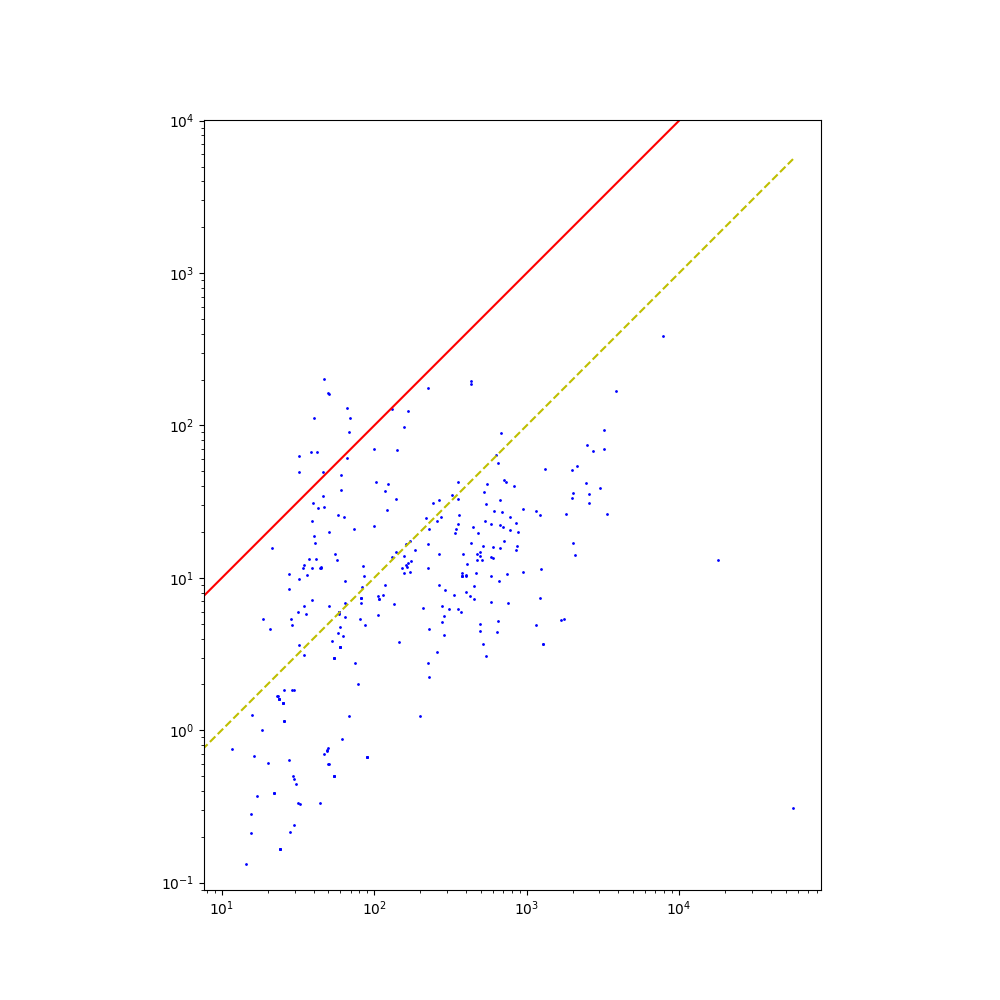
\includegraphics[width=0.35\textwidth,
                    trim=32mm 15mm 15mm 20mm] 
     {colors/gfx/normsize-no_cmemo.png}
     };
  \node(opt)[right=10mm of mono, inner sep=0] {
   \includegraphics[width=0.35\textwidth,
                    trim=32mm 15mm 20mm 20mm] 
     {colors/gfx/normsize-colored.png}
     };
  \node[below=-1mm of mono] {\axislab{separate e-graphs}};
  \node[left=-3mm of mono, rotate=90, anchor=south] {\axislab{monochrome colored e-graphs}};
  \node[below=-1mm of opt] {\axislab{separate e-graphs}};
  \node[left=-3mm of opt, rotate=90, anchor=south] {\axislab{optimized colored e-graphs}};
  \node(a)[right=10mm of opt] {$\times 1$};
  \node(b)[below=10mm of a.west,anchor=west] {$\times 10$};
  \draw[red,line width=0.8pt] (a.west) -- ++(-1, 0);
  \draw[yellow!50!gray,line width=1pt,dash pattern=on 2pt off 1pt] (b.west) -- ++(-1, 0);
\end{tikzpicture}
  %\includegraphics[width=0.3\textwidth]{gfx/normsize-colored.png}
  %\end{tabular}
  \vspace{-1em}
  \caption{Size comparison: relative e-node overhead in clones \vs color e-graph variants.}
  \label{fig:normalizedsize}
  \vspace{0.5em}
\end{figure*}

In our setup, all assumptions emerge from case splits done by the prover.
We filter out cases where no case splits were applied, since these have no assumptions introduced and thus colored e-graphs have no impact.

For each benchmark instance, we measure the \emph{relative e-node overhead} as the number of additional e-nodes that are required, normalized by the number of different assumptions.
That is, $(|\textrm{total e-nodes}| - |\textrm{base e-nodes}|) / |\textrm{assumptions}|$.
``Base e-nodes'' represent the contents of the graph before case splits.
(For the monochrome colored e-graph we use the base e-nodes present in the separate e-graphs case.)
\autoref{fig:normalizedsize} summarizes the results, pitting colored e-graphs (with and without colored e-nodes) against the baseline of separate clones.
In some cases one configuration times out or runs out of memory, while the other does not;
we only compare cases where both configurations finished the run successfully.
In both comparisons, we see roughly around 10$\times$ lower overhead, where in the monochromatic case samples are more dispersed around the y axis, and the optimized case shows clear advantage to the colored e-graph implementation.


Run-time is measured as the the total run-time for completed test cases, and 1 hour for cases that timed out.
We do not include runs that did not finish due to out-of-memory exceptions (we report the latter separately).
As can be seen in \autoref{fig:runtime}, the monochrome colored e-graph lead to many timeouts,
whereas the optimized case exhibits running times similar to separate clones.
This is in line with our expectation:
colors provide lower memory sizes at the expense of run-time.

\begin{figure*}
  \centering
  \newcommand\axislab[1]{\fontsize{7pt}{9pt}\selectfont{#1}}
\begin{tikzpicture}
  \node(mono)[inner sep=0] {
   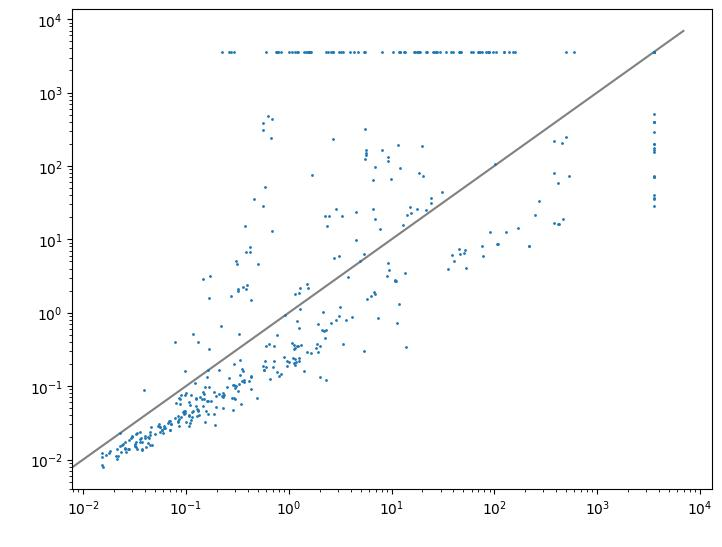
\includegraphics[width=0.35\textwidth, trim=20 20 20 15] 
     {colors/gfx/runtime-no_cmemo.jpg}
     };
  \node(opt)[right=12mm of mono, inner sep=0] {
   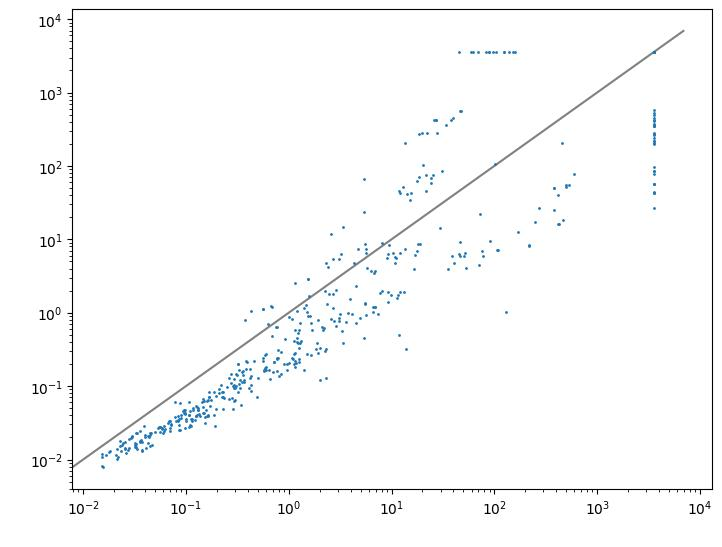
\includegraphics[width=0.35\textwidth, trim=20 20 20 15] 
     {colors/gfx/runtime-colored.jpg}
     };
  \node[below=0mm of mono] {\axislab{separate e-graphs}};
  \node[left=0mm of mono, rotate=90, anchor=south] {\axislab{monochrome colored e-graphs}};
  \node[below=0mm of opt] {\axislab{separate e-graphs}};
  \node[left=0mm of opt, rotate=90, anchor=south] {\axislab{optimized colored e-graphs}};
\end{tikzpicture}
    \vspace{-1em}
    \caption{Run-time comparison: run-time of clones vs. color e-graphs}
    \label{fig:runtime}
\end{figure*}

Finally, in \autoref{tab:runtimesuite} we present the number of out-of-memory exceptions, the number of timeout exceptions, and total run-time for each configurations and test suite.
The monochrome colored e-graph, as expected, exhibits many timeouts. 
Even though it has more errors than the other e-graph versions, it still has much longer run-times.

The optimized e-graphs demonstrate enhancements over separate e-graphs in both run-time and success rate, as detailed in \autoref{tab:runtimesuite}. 
Notably, the optimized configuration completed more tests (99 failures compared to 114). 
A key shift observed is the replacement of out-of-memory errors with timeouts, particularly in the \funcname{leon-amortize-queue} suite. 
However, \funcname{leon-heap} posed challenges for colored e-graphs, incurring 13 extra timeouts even in the optimized version. 
Conversely, the \funcname{isaplanner} suite showed a notable improvement, halving the failure rate in the optimized version compared to the baseline.

% I have a problem in how I test this, because it requires to assert both cases finished running and I can't do that at the moment
\begin{comment}
The \funcname{isaplanner} test suite contains a similar disparity, where for 79 test cases the colored e-graph has more assumptions by the end of the run.
There are no cases in \funcname{isaplanner} where the colored e-graphs had fewer assumptions, and there are only 4 test cases for which colored e-graphs had more assumptions in \funcname{leon-heap}, and none in which it had fewer.
\end{comment}


\begin{table}[t]
    \centering
    \caption{Run-time and exceptions. M = Out of memory, T = Timeout (3600) }
    \label{tab:runtimesuite}
    \setlength{\tabcolsep}{3pt} % Adjust the space between columns
    \newcolumntype{d}[1]{D{/}{/}{#1}} % New column type for O/T column
    \begin{tabular}{lrd{3}rd{3}rd{3}}
    \toprule
    & \multicolumn{2}{c}{Separate} & \multicolumn{2}{c}{Monochrome} & \multicolumn{2}{c}{Optimized} \\
    \cmidrule(r){2-3} \cmidrule(lr){4-5} \cmidrule(l){6-7}
    Test Suite & \multicolumn{1}{c}{Time} & \multicolumn{1}{l}{M/T} & \multicolumn{1}{r}{Time} & \multicolumn{1}{l}{M/T} & \multicolumn{1}{r}{Time} & \multicolumn{1}{l}{M/T} \\
    \midrule
    clam & 70.1 & 0/0 & 277.8 & 0/5 & 23.6 & 0/0 \\
    hipspec-rev-equiv & 34.1 & 0/0 & 139.0 & 0/17 & 57.0 & 0/0 \\
    hipspec-rotate & 3880.3 & 1/1 & 1871.4 & 0/6 & 17.4 & 0/3 \\
    isaplanner & 8454.4 & 0/60 & 6068.4 & 0/70 & 20486.3 & 3/28 \\
    leon-amortize-queue & 187356.4 & 52/0 & 14.8 & 0/57 & 10854.3 & 3/49 \\
    leon-heap & 1735.9 & 0/0 & 1201.8 & 0/25 & 4949.2 & 0/13 \\
    \bottomrule
    \end{tabular}
\end{table}







\begin{comment}
    \begin{tabular}{llr}
\toprule
 &  & Time \\
E-graph Type & Test Suite &  \\
\midrule
\multirow[t]{7}{*}{Seperate e-graphs} & clam & 34.234764 \\
 & hipspec-nichomachus & 0.050861 \\
 & hipspec-rev-equiv & 2.577174 \\
 & hipspec-rotate & 237.717540 \\
 & isaplanner & 8913.695004 \\
 & leon-amortize-queue & 9.668328 \\
 & leon-heap & 216.857437 \\
\cline{1-3}
\multirow[t]{7}{*}{Monochromatic colored e-graphs} & clam & 394.891332 \\
 & hipspec-nichomachus & 0.087772 \\
 & hipspec-rev-equiv & 0.720120 \\
 & hipspec-rotate & 1970.451256 \\
 & isaplanner & 1739.190107 \\
 & leon-amortize-queue & 0.294397 \\
 & leon-heap & 1206.035020 \\
\cline{1-3}
\multirow[t]{7}{*}{Optimized colored e-graphs} & clam & 6.049511 \\
 & hipspec-nichomachus & 0.085397 \\
 & hipspec-rev-equiv & 42.016671 \\
 & hipspec-rotate & 78.174158 \\
 & isaplanner & 12337.053032 \\
 & leon-amortize-queue & 43.787478 \\
 & leon-heap & 791.375722 \\
\cline{1-3}
\bottomrule
\end{tabular}
\end{comment}
\section{Related Work}
\label{colors:related}

\myparagraph{Theory exploration and its applications.}
Interest in exploratory reasoning in the context of functional calculi started with IsaCoSy~\cite{JAR2010:Johanssonisacosy}, a system for lemma discovery based in part on CEGIS~\cite{ASPLOS2006/Solar-Lezama}.
In a seminal paper, QuickSpec~\cite{JFP2017:Smallbone}
propelled applicability of such reasoning for inferring specifications from implementations
based on random testing,
with deductive reasoning to verify generated conjectures~\cite{ICAD2013:Claessen,ITP2017:Johansson}.
TheSy~\cite{thesy} and Ruler~\cite{ruler} have both incorporated e-graphs to some extent in the exploration process: they are used to speed up equivalence reduction of the space of generated terms, and, in~\cite{thesy}, also the filtering and qualification phases using symbolic examples.
The evaluation of the latter shows quite clearly that case splitting is a major obstacle to symbolic exploratory reasoning,
due to the large number of different cases and derived assumptions.

In the area of conditional rewrite discovery,
Speculate~\cite{speculate}
naturally builds on the techniques from QuickSpec and depends on property-based testing techniques to generate inputs that satisfy some conditions.
SWAPPER~\cite{DBLP:conf/fmcad/0002S16} is a relatively early example of exploring using SyGuS with a data-driven inductive-synthesis approach with emphasis on finding rules that are most efficient for different problem domains.
It requires a large corpus of similar SMT problems to operate.

%QuickSpec etc (from TheSy and others), Ruler, SWAPPER, Speculate, Spectacular
%Case splitting in hipspec and conditions in Speculate

\myparagraph{Other e-graph extensions.}
E-graphs were originally brought into use for automated theorem proving~\cite{JACM2005:Detlefs},
and were later popularized as a mechanism for implementing low-level compiler
optimizations~\cite{POPL2009:Tate},
by extending them with ``$\varphi$-nodes'' to express loops.
Relational e-matching~\cite{DBLP:journals/pacmpl/ZhangWWT22}
makes use of Datalog semina\"ive evaluation
to harness the power of query planning in database systems.
Subsequently, Datalog-powered e-matching has been recently fused with core Datalog semantics to allow richer logic programming by exposing equality saturation as a building block in a framework called egglog~\cite{DBLP:pldi23/Zhang}.
Since Datalog is based on Horn clauses, this meshes very well with conditional rewriting.
It should be noted, though, that it is still a monotone framework, and does not allow backtracking or simultaneous exploration of alternative assumptions.

ECTAs~\cite{Koppel22,Koppel23} are another, related compact data structure that extends e-graphs, Version-Space Algebras~\cite{DBLP:conf/icml/LauDW00,DBLP:journals/ml/LauWDW03}, and Finite Tree Automata~\cite{DBLP:journals/pacmpl/0001M17},
with the concept of ``entanglement'';
that is, some choices of terms from e-classes
may depend on choices done in other e-classes.
Since the backbone of ECTAs is quite similar to an e-graph, the colors extension is applicable to this domain as well.

\myparagraph{Uses of e-graphs in SMT.}
E-graphs are a core component for equality reasoning in SMT solvers~\cite{z3,DBLP:conf/tacas/BarbosaBBKLMMMN22}, in most theory solvers such as QF\_UF, linear algebra, and bit-vectors.
E-matching is also used for quantifier instantiation~\cite{DBLP:conf/tacas/NiemetzPRBT21}, which is, in its essence, an exploratory task and requires efficient methods~\cite{DBLP:conf/cade/MouraB07}.
In these contexts, implications and other Boolean structures are treated by the SAT core (in CDCL(T)), and the theory solver only handles conjunctions of literals.

\section{Conclusion}
\label{colors:conclusions}
% We created colored e-graphs for multiple congruence relations
% We evaluated and it is good


% We want future work


\begin{comment}
In conclusion, this paper has introduced the concept of colored e-graphs as a memory-efficient method for maintaining multiple congruence relations in a single e-graph. 
It provides support for equality saturation with additional assumptions over e-graphs, thereby enabling efficient exploratory reasoning of multiple assumptions simultaneously.
The development of several optimizations based on the egg library and deferred rebuilding, and subsequent evaluation has validated our approach, demonstrating a significant improvement in memory utilization and a modest one for run-time performance compared to the baseline.
\end{comment}

We presented colored e-graphs as an approach to efficiently handle multiple congruence relations in a single e-graph.
They provide a memory-efficient method for equality saturation with additional assumptions, crucial for efficient exploratory reasoning of multiple assumptions simultaneously.
Our optimizations, developed using the egg library, have shown notable improvements in memory usage and moderate enhancements in run-time performance over the baseline.

%This work thus serves as a stepping stone, advancing the current state of the art and setting a foundation for works on exploratory reasoning tools and techniques. 
%By extending e-graph capabilities, we hope to drive new innovation in the realm of symbolic reasoning and its applications.

\clearpage

\bibliographystyle{splncs04}
\bibliography{bib}
\clearpage

%\appendix
\begin{appendices}
\section{Background on E-graphs}
\label{background}

% The following went into chatgpt
% An E-Graph needs to support Adding E-Nodes, a union operation, E-Matching, and keeping congruence closure. egg [citetion] added changed how we use E-Graphs by expressivly supporting the equality saturation workflow. They did this by only holding congruence closure at certain points in the run, allowing us to amortize the costs of rebuilding the closure.
% In this work, we are further expanding on equality saturation. In our use case, the E-Graph is used for equality saturation, in an automatic reasoning set up, where there is a need to reason about multiple cases, or multiple equivalence relations at once. In this setting we want to again amortize the costs, but this time improve the memory usage of the E-Graph, by reusing as many parts as possible. To better understand this point, we first explain what are the main data structures used by egg. 
% As mentioned in egg [citation], it is useful to think about an E-Graph as an extension of union-find, to support expressions. The main operations of the E-Graph, that is supporting the extended union-find, are implemented using a union-find, equality class (E-Class) map, and hash-cons. The union-find is used to track the equality classes, while the E-Class map and hash-cons are used for supporting the "expressions" part. The expression support is actually two fold, first we need to support addition, and second we need to support congruence closure. Addition is supported using the hash-cons which is a memorization of the expressions (E-Nodes) and what is their containing E-Class. The congruence closure is done during "rebuild" where the E-Class map (and their parents) are used in conjunction with the hash-cons to find E-Classes that should be merged.
% There is the additional E-Matching that needs support for equality saturation, but that is implemented over the E-Class map with an additional hash-map for expression operation to class-ids for performance.

We will now present some general background on e-graphs.
Same as in \autoref{overview}, we assume a term language $L$ where terms are constructed using \emph{function symbols}, each with its designated arity.
We use $f^{(r)}\in\Sigma[L]$ to say that $f$ is
in the \emph{signature} of $L$ and has arity $r$.

An e-graph $\mathcal{G}$ serves as a compact data structure representing a set $S\subseteq L$ of terms and a congruence relation ${\cong}\subseteq L\times L$. This congruence relation, in addition to being reflexive, symmetric, and transitive, is also closed under the function symbols of $\Sigma[L]$. That is, for every $f^{r}\in\Sigma[L]$, and given two lists of terms $t_{1..r}\in L$ and $s_{1..r}$, each of length $r$, if $t_i\cong s_i ~ (i=1..r)$, then it follows that $f(t_1,\ldots,t_r)\cong f(s_1,\ldots,s_r)$. This property, known as \emph{congruence closure}, is a key attribute of the data structure. The maintenance of this attribute as an invariant significantly influences the design and implementation of e-graph actions.

The egg library~\cite{egg} revolutionizes the application of e-graphs by explicitly supporting the equality saturation workflow.
It enables the periodic maintenance of congruence closure, via \emph{deferred rebuild}, allowing for the amortization of associated rebuilding costs.
%We give a short background on how egg achieves better performance by means of efficient data structure representation.

In egg, the authors present the e-graph as a union-find-like data structure, augmented to support operations on expressions.
This implementation is primarily achieved through the utilization of three key structures: a hash-cons table, a union-find structure, and an e-class map.
These structures collectively underpin the functionalities integral to the operation of the e-graph.

\begin{enumerate}[(a)]
%
% Union find
\item The \underline{union-find} component is responsible for keeping track of merged e-classes and maps each e-class id to a single representative for all (transitively) merged e-classes.
This information is later used to canonicalize the keys and values of the hash-cons.
%
% E-Class map
\item The \underline{e-class map} stores the structure of the e-graph.
For each e-class id, the map keeps all the e-nodes that are contained therein.
E-nodes are similar to AST nodes except that their children point to e-class ids instead of containing a single sub-term each.
%Through the contained e-nodes, child e-classes can be reached. 
%For efficiency, the e-graph also keeps the parents of each e-class,
%i.e., those of whose it is a child of.
%
% Hash-Cons
\item The \underline{hash-cons} table maps e-nodes to their containing e-class id.
An important aspect of the hash-cons is that after rebuilding, its keys and values are expected to be \emph{canonical}. 
That is, whenever e-classes are merged one of their ids becomes ``the'' representative.
%A \emph{canonical} hash-cons will only contain representative ids.
%For example, if $x$ and $y$ are merged into $y$, then $f(x,z) \mapsto x$ must become $f(y,z) \mapsto y$.
\end{enumerate}

%Note, that both the hash-cons and the parent e-classes can be derived from the e-nodes contained in the e-class map.
%But, they are important aspects of the efficient e-graph implementation presented, and therefore are mentioned as part of the data structure.

An e-class with id $e$ represents a set of terms defined recursively as:
\begin{align*}
L(e) &= \{f(t_1,..,t_k)~|~ \\ 
     & \qquad f(e_1,..,e_k)\in M(e), t_i\in L(e_i)\mbox{~for~}i=1..k\}
\end{align*}
We will use the notation $[t]$ to refer to e-class id where $t\in L([t])$.

\begin{example}
The terms $\tmax(x, y)$ and $x - y$ are both represented in the e-graph in \autoref{overview:egraph-max}(a) using e-classes $\ecid5$ and $\ecid6$, respectively, with  the following e-nodes:
%
\[
M \quad = \quad
\adjustbox{valign=t}{
$
\begin{array}{@{}ll}
  \ecid1 \mapsto \{\ttrue\} & \ecid2 \mapsto \{\tfalse\} \\
  \ecid3 \mapsto \{x\} & {} \ecid4 \mapsto \{y\} \\
  \ecid5 \mapsto \{\tmax(\ecid3, \ecid4)\} & \ecid6 \mapsto \{\ecid3 - \ecid4\}
\end{array}
$
}
\]

\begin{comment}
The e-graph maintains a union-find, which, in this trivial example, is a bit boring since it is an identity relation.

The contents of the hash-cons (which can be easily discerned by inverting $M$) are:
\[H \quad = \quad a \mapsto \ecid1 \quad b\mapsto \ecid2 \quad 
   c\mapsto \ecid3 \qquad
  \ecid2 + \ecid3 \mapsto \ecid4 \qquad \ecid1 \cdot \ecid4\mapsto \ecid5\]
\end{comment}

\end{example}

An e-graph where every e-class is a singleton, like this one, is just a forest of expression trees with sharing.
The situation becomes more interesting once we start mutating the graph via its dedicated operations.

% Functionalities
\begin{enumerate}
% (1) Insert
\item \underline{Insert} - Adds a term $t$ to the e-graph, one e-class per AST node, reusing e-classes where possible by searching the hash-cons.
% (2) Union
\item \underline{Merge} - Merging two e-classes by applying a union operation of the union-find and merging the classes in the e-class map.
This, however, temporarily invalidates the invariant of the hash-cons and e-class map that all e-class ids and e-nodes must be canonical.
% (3) Congruence closure
\item \underline{Rebuilding (Congruence closure)} - As explained before, a union of $[x]$ into $[y]$ necessitates replacing any e-node $f([x],[z])$ by $f([y],[z])$.
Moreover, if $f([x],[z])\in[w_1], f([y],[z])\in[w_2]$,
then, following this replacement, both $[w_1]$ and $[w_2]$ now contain
$f([y],[z])$, meaning that $[w_1] = [w_2]$ and evoking a cascading union of $[w_1], [w_2]$.
A significant contribution by egg is the concept of deferred (and thus periodic) rebuilding.
This periodic rebuilding is highly efficient and well-suited for equality saturation.
% (4) E-matching
\item  \underline{E-matching} - Looking up a \emph{pattern} in the set of terms represented by the e-graph in a top-down manner, traversing the e-nodes downward via the e-class map.
A pattern is a term with (zero or more) \emph{holes} represented by metavariables $?v_{1..k}$.
For example, $(?v_1+1)\cdot ?v_2$ is a pattern.
Pattern lookup is important for rewriting in equality saturation.
\end{enumerate}

\smallskip
\noindent\textbf{Rewriting.~}
We assume a background set of symbolic \emph{rewrite rules} (r.r.), each of the form $t\rwto s$,
where $t$ and $s$ are patterns as explained in item (4) above.
A \emph{match} $\theta$ of pattern $t$ on the e-graph, is an assignment mapping metavariables to e-class ids.
$t\theta$ represents an e-node, and we will denote its equality class as $[t\theta]$.
Applying the r.r. is done by merging the e-classes $[s\theta]$ and $[t\theta]$. 
Because the e-node $s\theta$ might be new, it needs to also be inserted, resulting in $union([t\theta], insert(s\theta))$.
Repetitively applying such rewrite rules to a set of terms can be used to generate growing sets of terms that are equivalent, according to rewrite semantics, to ones in the starting set.
Ideally, the set eventually \emph{saturates}, in which case the e-graph now describes \emph{all} the
terms that are rewrite-equivalent.
We point out that in many situations, the e-graph keeps growing as a result of rewrites and never gets saturated---so the number of successive rewrite iterations, or ``rewrite depth'', has to be bounded.

A \emph{conditional rewrite rule} (c.r.r.)~\cite{jcss/Bergstra} is a natural extension of a r.r. that has the following form:
$\varphi \Rightarrow t \rwto s$
where $\varphi$ is a precondition for rewriting $t$ to $s$. For example, the rules for $max$ are:
${?x} > {?y} \Rightarrow \tmax({?x}, {?y}) \rwto {?x}$ and 
${?x} \leq {?y} \Rightarrow \tmax({?x}, {?y}) \rwto {?y}$.
%
The semantics of a precondition $\varphi$ is defined such that a term matching the pattern of $\varphi$
must be unified with Boolean $\ttrue$ in order for the rewrite to be applied.

\chapter{Algorithms Pseudo Code}
\label{app:algorithms}

Colored e-graphs introduce a few algorithmic changes to the operations of a normal e-graph.
Here we present pseudo code for the important changes presented in the paper.
Algorithms \ref{alg:compare} and \ref{alg:colored_jump} present the changes being made to the e-matching abstract machine to support \emph{unoptimized} colored e-matching as presented in \autoref{colors:functional}.

\begin{algorithm}
\caption{Function: compare}
\label{alg:compare}
\begin{algorithmic}
\STATE \textbf{Input:} $i$, $j$
\IF{$find(color, reg[i]) \neq find(color, reg[j])$}
    \STATE \textbf{backtrack}
\ENDIF
\end{algorithmic}
\end{algorithm}

\begin{algorithm}
\caption{Function: colored\_jump}
\label{alg:colored_jump}
\begin{algorithmic}
\STATE \textbf{Input:} $i$
\STATE $siblings \gets \{e | e \in E \land e \equiv_{color} eclass\}$
\FOR{$sibling$ in $siblings$}
    \STATE $reg[i] = sibling$
    \STATE $bs$.push(current\_state)
\ENDFOR
\STATE \textbf{backtrack}
\end{algorithmic}
\end{algorithm}

The rebuilding algorithm is also updated to accommodate for colored e-graphs in \autoref{colors:functional}.
We update the auxiliary function \textsc{repair} to work on colored e-classes,
and introduce two new helper functions: $\textsc{collect\_parents}$ and $\textsc{update\_hashcons}$, as presented in Algorithms \ref{alg:rebuild}, \ref{alg:repair}, \ref{alg:update_hashcons}, and \ref{alg:collect_parents}.
$\textsc{collect\_parents}$ extract the parents of a colored e-class by combining the sets of parents of all the (root) e-classes contained therein.
$\textsc{update\_hashcons}$ is used to make sure that the hashcons entries are in canonical forms. It was already a part of \textsc{repair} in egg;
it is only repeated here to point out that it
only updates the hashcons for the root color,
since no canonization is required for colored layers.    

\begin{algorithm}
\caption{Function: rebuild}
\label{alg:rebuild}
\begin{algorithmic}
\FOR{$color$ in $self.colors$}
    \WHILE{$self.worklist(color).len() > 0$}
        \STATE $todo \gets$ TAKE($self.worklist(color)$)
        \STATE $todo \gets \{ self.find(color, eclass) | eclass \in todo \}$
        \FOR{each $eclass$ in $todo$}
            \STATE CALL $self.repair(color, eclass)$
        \ENDFOR
    \ENDWHILE
\ENDFOR
\end{algorithmic}
\end{algorithm}

\begin{algorithm}
\caption{Function: repair}
\label{alg:repair}
\begin{algorithmic}
\STATE \textbf{Input:} $color$, $eclass$
\STATE $parents \gets$ CALL collect\_parents($color, eclass$)
\STATE CALL update\_hashcons($color, parents$)
\STATE $new\_parents \gets \{\}$
\FOR{each $(p\_node, p\_eclass)$ in $parents$}
    \STATE $p\_node \gets self.canonicalize(color, p\_node)$
    \IF{$p\_node$ is in $new\_parents$}
        \STATE $self.merge(color, p\_eclass, new\_parents[p\_node])$
        \STATE $new\_parents[p\_node] \gets self.find(color, p\_eclass)$
    \ENDIF
\ENDFOR
\IF{$color = root$}
    \STATE $eclass.parents \gets new\_parents$
\ENDIF
\end{algorithmic}
\end{algorithm}

\begin{algorithm}
\caption{Function: update\_hashcons}
\label{alg:update_hashcons}
\begin{algorithmic}
\STATE \textbf{Input:} $color$, $parents$
\IF{$color = root$}
\FOR{each $(p\_node, p\_eclass)$ in $parents$}
    \STATE $self.hashcons.remove(p\_node)$
    \STATE $p\_node \gets self.canonicalize(color, p\_node)$
    \STATE $self.hashcons[p\_node] \gets self.find(color, p\_eclass)$
\ENDFOR
\ENDIF
\end{algorithmic}
\end{algorithm}

\begin{algorithm}
\caption{Function: collect\_parents}
\label{alg:collect_parents}
\begin{algorithmic}
\STATE \textbf{Input:} $color$, $eclass$
\STATE $all\_parents \gets \emptyset$
\STATE $relevant\_eclasses \gets \{e | e \in E \land e \equiv_{color} eclass\}$
\FOR{$e$ in $relevant\_eclasses$}
    \STATE $all\_parents \gets all\_parents \cup e.parents$
\ENDFOR
\STATE return $all\_parents$
\end{algorithmic}
\end{algorithm}

The pseudo code for the optimized e-matching instructions that were presented in \autoref{colors:optimizations} are presented in Algorithms \ref{alg:compare_optimized} and \ref{alg:colored_jump_optimized}.

\begin{algorithm}
\caption{Function: compare' (optimized)}
\label{alg:compare_optimized}
\begin{algorithmic}
\STATE \textbf{Input:} $i$, $j$
\IF{$find(color, reg[i]) \neq find(color, reg[j])$}
    \STATE $descendants \gets \{ c | color \in p^+(c) \land reg[i] \equiv_c reg[j] \}$
    \STATE $minimal \gets \{ c | c \in descendants \land \lnot \exists c' \in descendants. c' \in p^+(c) \}$
    \FOR{$c$ in $minimal$}
        \STATE $color = c$
        \STATE $bs$.push(current\_state)
    \ENDFOR
    \STATE \textbf{backtrack}
\ENDIF
\end{algorithmic}
\end{algorithm}

\begin{algorithm}
\caption{Function: colored\_jump' (optimized)}
\label{alg:colored_jump_optimized}
\begin{algorithmic}
\STATE \textbf{Input:} $i$
\STATE $siblings \gets \{e | e \in E \land e \equiv_{color} eclass\}$
\FOR{$sibling$ in $siblings$}
    \STATE $reg[i] = sibling$
    \STATE $bs$.push(current\_state)
\ENDFOR
\STATE $descendants \gets \{ (c, e) | color \in p^+(c) \land reg[i] \equiv_c e \land e \notin siblings \}$
\STATE $minimal \gets \{ (c, e) | (c, e) \in descendants \land \lnot \exists (c', e') \in descendants. (c' \in p^+(c) \land e' \equiv_c' e) \}$
\FOR{$(c,e)$ in $minimal$}
    \STATE $color = c$
    \STATE $reg[i] = e$
    \STATE $bs$.push(current\_state)
\ENDFOR
\STATE \textbf{backtrack}
\end{algorithmic}
\end{algorithm}
\newpage
\newpage
\clearpage
\section{Walkthrough for Example 2}
\label{app-b}

This is the full walkthrough of the example in \autoref{overview:egraph-max} from the overview.

We walk through the steps needed to carry out the case splitting shown in \autoref{overview:egraph-max-min}.
The system contains the conditional rewrite rules shown on the right of \autoref{app-b:colored:example}, which 
constitute the definitions of $\tmax$ and $\tmin$,
plus some prior knowledge about $|\,{\cdot}\,|$ and $-$.

\newcolumntype{L}[1]{>{\raggedright\let\newline\\\arraybackslash\hspace{0pt}}m{#1}}

\begin{figure*}[t]
\begin{center}
\begin{tabular}{ll}
\begin{tabular}{L{3.5cm}l@{}}
    {\small (1)}\newline
    merge$\lowerred$($[x < y]$, $[\tfalse]$)
    &
    \raisebox{-0.5\totalheight}{\fbox{
      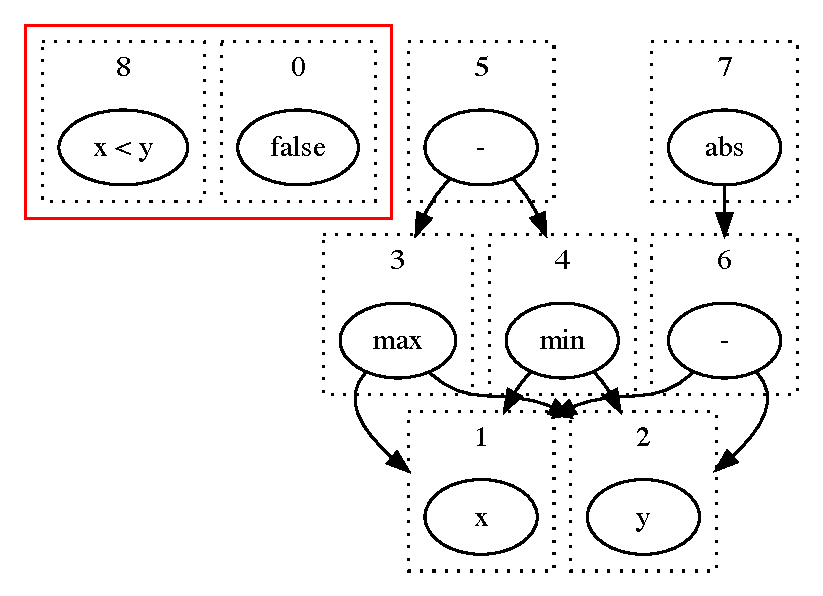
\includegraphics[width=4cm]{gfx/example_graphs_res/00-init.pdf}
    }}
    \\
    {\small (2)}\newline
    merge$\lowerred$($[\tmax(x, y)]$, $[x]$)\newline
    merge$\lowerred$($[\tmin(x, y)]$, $[y]$)\newline
    merge$\lowerred$($[|x - y|]$, $[x - y]$)
    &
    \raisebox{-0.5\totalheight}{\fbox{
      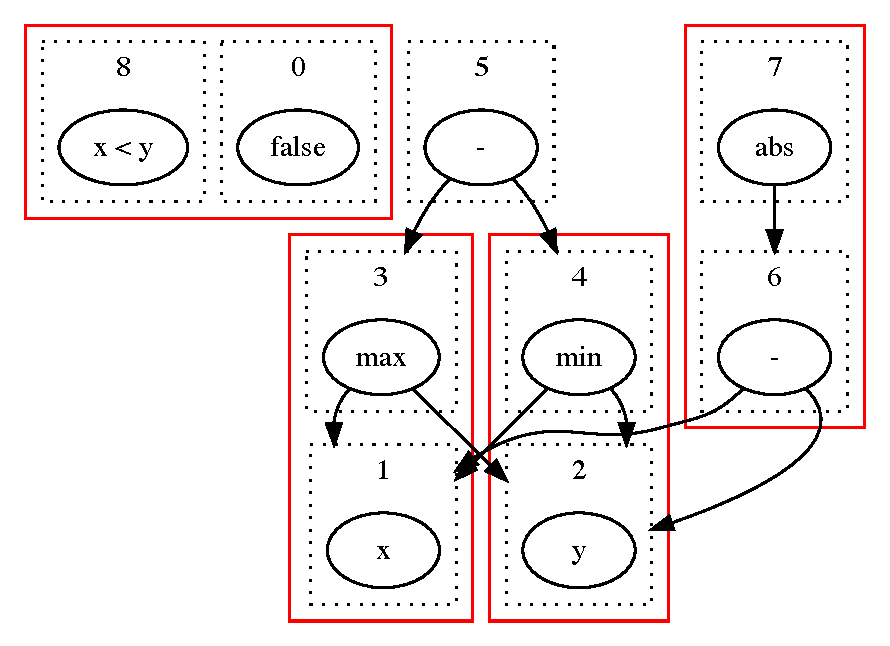
\includegraphics[width=4cm]{gfx/example_graphs_res/01-after_rw.pdf}
    }}  
    \\
    {\small (3)}\newline
    rebuild$\lowerred$() \newline
    \quad $\downarrow$ \newline
    merge$\lowerred$($[x - y]$, \newline
    \hspace{3em} $\tmax(x) - \tmin(y)$)
    &
    \raisebox{-0.5\totalheight}{\fbox{
    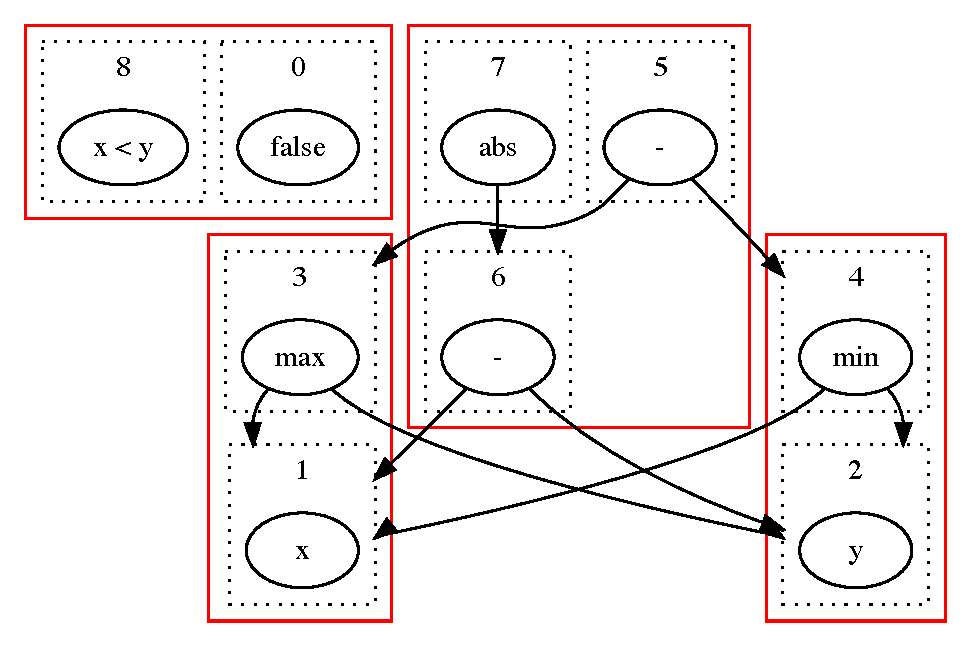
\includegraphics[width=4cm]{gfx/example_graphs_res/02-final.pdf}
    }}

\end{tabular}
%
&
\scalebox{0.9}{
$\begin{array}{c}
        \mbox{rewrite rules} \\ \arrayrulecolor{gray!50!white}\hline
        {?x} < {?y} \Rightarrow \tmin({?x}, {?y}) \rwto {?x} \\
        \lnot{?x} < {?y} \Rightarrow \tmin({?x}, {?y}) \rwto {?y} \\
        {?x} < {?y} \Rightarrow \tmax({?x}, {?y}) \rwto {?y} \\
        \lnot{?x} < {?y} \Rightarrow \tmax({?x}, {?y}) \rwto {?x} \\
        {?x} < {?y} \Rightarrow |{?x} - {?y}| \rwto {?y} - {?x} \\
        \lnot{?x} < {?y} \Rightarrow |{?x} - {?y}| \rwto {?x} - {?y} \\
    \end{array}$
}
\end{tabular}
%    
\caption{\label{app-b:colored:example}
    Rewriting with case-split in a colored e-graph.}

\end{center}
\end{figure*}

The semantics of a conditional rewrite rule in the domain of an e-graph is that the condition pattern should be matched and its root must be in the same e-class as $\ttrue$, and, additionally, the left-hand side should be matched as normal.
For simplicity of presentation, we pretend that $\lnot$ is a special case were the negated condition is e-matched and the e-class should contain $\tfalse$.

\smallskip
Starting with the base graph, \autoref{overview:egraph-max-min}(a), we describe the operation of Easter Egg
on the \cred color, corresponding to the case $\lnot x < y$.
The complement \cblue case ($x < y$) is analogous.

\begin{enumerate}[leftmargin=1.5em]
\item
    The value of $x < y$ is declared as $\tfalse$ via
    a colored merge.
    This yields a new \cred e-class.
\item
    Colored e-matching is performed against the premise of the c.r.r. $\lnot {?x} < {?y} \Rightarrow \tmax({?x}, {?y}) \rwto {?x}$.
    The condition of the rule, ${?x} < {?y}$, matches against the class $[x < y]$, 
    which is indeed in the same \cred e-class as $\tfalse$.
    
    Similar e-matches are carried out for the rules
    $\lnot {?x} < {?y} \Rightarrow \tmin({?x}, {?y}) \rwto {?y}$
    and
    $\lnot {?x} < {?y} \Rightarrow |{?x} - {?y}| \rwto {?x} - {?y}$.
\item
    The children of $\ecid3 - \ecid4 ~(\in M(\ecid5))$ are \cred-equivalent to those of $\ecid1 - \ecid2 ~(\in M(\ecid6))$, and,
    as a consequence, \cred congruence closure kicks in and performs a \cred union there.
\end{enumerate}

\medskip
The process for \cblue is analogous.
The case-split semantics is defined such that it records the fact
that \cblue and \cred are \emph{complements},
and as such extends $\equiv$ with the common equivalences,
$\congblue\cap\congred = \big\{\big\langle\ecid5,\ecid7\big\rangle, \ldots\big\}$.
\end{appendices}
\end{document}



